% ==============================================================================
\chapter{Semiconductor detectors for radiation detection}
\label{sec:SiliconTheory}
%==============================================================================    

%% --------------------------------------------- %%
\section{Intrinsic silicon}
Due to periodic lattice of crystalline structure of semiconductor
material, electrons within the solid have allowed energy bands. The
energy of the electrons is confined to one of the energy bands. The
bands may be separated by ranges of forbidden energies.

\begin{figure}[htbp]
  \centering
  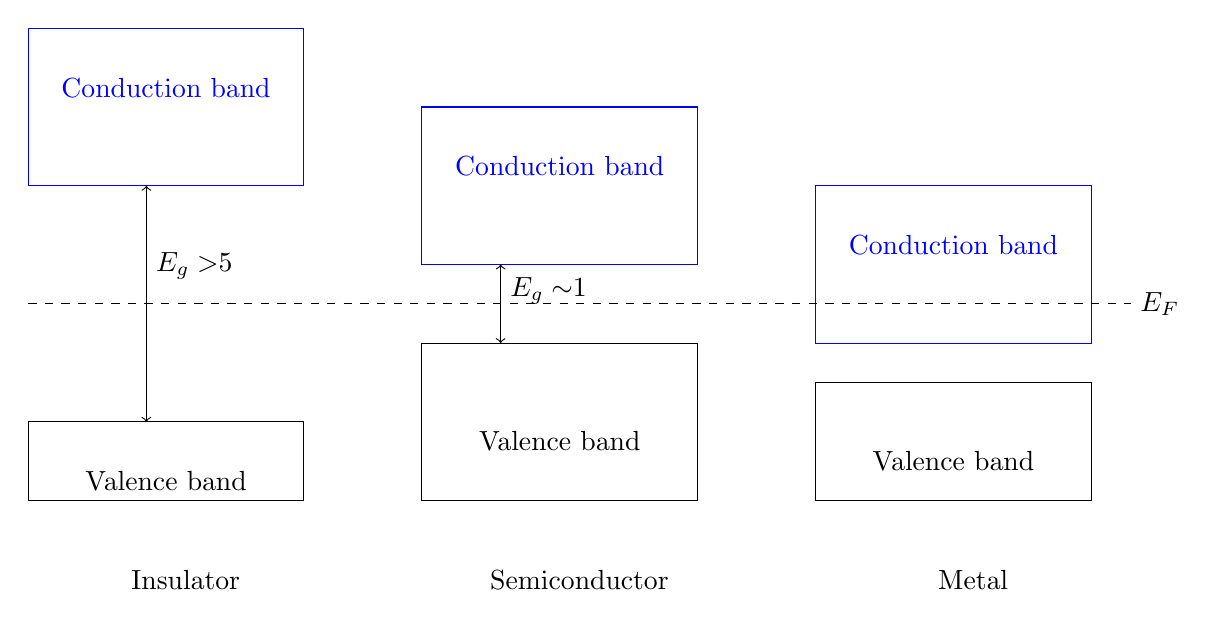
\begin{tikzpicture}
    \begin{scope} % Valence and conduction bands
      %  ----- insulator ----- %
        \draw (0, 1) rectangle node[below] {Valence band}  ++ (3.5, 1);
        \draw[blue] (0, 5) rectangle node[above] {Conduction band} ++ (3.5, 2);
        \node at (2, 0) {Insulator};

        % ----- Semiconductor ----- %
        \draw (5, 1) rectangle node[below] {Valence band}  ++ (3.5, 2);
        \draw[blue] (5, 4) rectangle node[above] {Conduction band} ++ (3.5, 2);
        \node at (7, 0) {Semiconductor};

        % ----- Metal ----- %
        \draw (10, 1) rectangle node[below] {Valence band}  ++ (3.5, 1.5);
        \draw[blue] (10, 3) rectangle node[above] {Conduction band} ++ (3.5, 2);
        \node at (12, 0) {Metal};
    \end{scope}


    \begin{scope} % Energy levels
        \draw[dashed] (0, 3.5) -- (14, 3.5) node[right] {$E_{F}$};
        \draw[arrows=<->](1.5, 2)--(1.5, 5) node [pos=0.66,right] {$E_{g}>$\SI{5}{\electronvolt}};
        \draw[arrows=<->](6, 3)--(6, 4) node [pos=0.66,right] {$E_{g}\sim$\SI{1}{\electronvolt}};
    \end{scope}

  \end{tikzpicture}
  \caption{}  \label{fig:energyBands}
\end{figure}

%% --------------------------------------------- %%
\section{Charge generation in silicon}

\subsection{Bethe-Bloch formula}
In silicon, free charge careers are generated due to thermal effects
and lead to leakage current. Charged particles are also detected by a
current generated due to their interaction with the sensor
material. Part of the absorbed energy generates electron-hole pairs
through scattering processes with the shell electrons of silicon and
can be collected by the readout electronic. The energy loss along the
particle track is described by the Bethe-Bloch
formula~\cite{Beringer:1900zz}.

\begin{equation}
  - \frac{dE}{dx} = 4 \pi N_A r_{e}^2 m_e c^2 z^2 \frac{Z}{A}  \frac{1}{\beta^2} \left[ \frac{1}{2} \ln{\frac{2 m_e c^2 \beta^2 \gamma^2 T_{max}}{I^2}} - \beta^2 - \frac{\delta}{2}\right]\; ,
  \label{eq:BetheBloch}
\end{equation}

where $z$ is the charge of the traversing particle, $Z$ the atomic
number, $A$ the atomic mass of the absorption medium, $m_ec^2$ the
rest energy of the electron, $\beta={v \over c}$,
$\gamma=1/\sqrt{1-\beta^2}$, $I$ the mean excitation energy and
$T_{max}$ the maximum kinetic energy that a particle can transfer to a
shell electron.  A minimum ionising particle (MIP) has an energy loss
in the minimum of the Bethe-Bloch formula. Relativistic particles are
considered as MIPs.

Ionisation is also subject to statistical fluctuations and
Equation~\ref{eq:BetheBloch} gives its average value. It can be
described by a probability density function called \textit{straggling
functions} and characterised by the most probable energy loss
($\Delta_{p}$) and full-width-at-half-maximum
($w$). Figure~\ref{fig:LandauDistribution} shows examples of this
distribution in thin sensors. If a particle is not stopped in the
sensors, the energy deposition varies around the peak of the
distribution and the average value is higher than the most probable
value ($\Delta_{p}$) of the distribution. The fluctuations around the
$\Delta_{p}$ increase for thinner sensors and should be taken into
account for the design of the dynamic range of the readout
electronics.


\begin{figure}[htbp]
  \centering
  \includegraphics[width=0.7\textwidth, page=14, trim = 50mm 160mm
  40mm 20mm, clip]{Articles/rpp2009-rev-passage-particles-matter.pdf}
  \caption{Straggling functions in silicon for 500 MeV pions,
    normalized to unity at the most probable value. $w$
    is the full-width-at-half-maximum~\cite{Beringer:1900zz}.}
  \label{fig:LandauDistribution}
\end{figure}

\subsection{Bichsel model}
Bichsel~\cite{Bichsel} provides a theory to calculate the
straggling functions and compares different methods. He also gives an
approximation of $\Delta_{p}$ and $FWHM$ as function of the thickness
$t$ of silicon detectors for particles with charge $\pm1e$ and
$\beta\gamma>500$ as listed in Equations~\ref{eq:MPV1}, \ref{eq:MPV2},
\ref{eq:FWHM}:

\begin{itemize}
\item For $13<t<110$ [micron]:
  \begin{equation}
    \Delta_{p}=t \cdot (100.6+35.35 \cdot \ln(t))\; ,
    \label{eq:MPV1}
  \end{equation}
\item For $110<t<3000$ [micron]:
  \begin{equation}
    \Delta_{p}=t \cdot (190+16.3 \cdot \ln(t))\; ,
    \label{eq:MPV2}
  \end{equation}
\item For $30<t<260$ [micron]:
  \begin{equation}
    FWHM=t \cdot (259.6-28.41 \cdot \ln(t)).
    \label{eq:FWHM}
  \end{equation}
\end{itemize}

Table~\ref{tab:EdepForDifferentThickness} summarises the $\Delta_{p}$
and $FWHM$ for detectors thicknesses at our disposal. 

\begin{table}[htbp]
  \centering
  \caption{$\Delta_{p}$ and $FWHM$ calculated for silicon sensors with
    different thicknesses using Equations~\ref{eq:MPV1}, \ref{eq:MPV2}
    and \ref{eq:FWHM}.}
  \label{tab:EdepForDifferentThickness}
  \begin{tabular}{c c c c}
    \toprule
    Thickness [micron] &  $\Delta_{p}$ [keV] & $FWHM$ [keV] & $\Delta_{p} / FWHM$ \\ 
    \midrule
    50 & 11.9 & 7.42 & 1.6      \\
    100 & 26.34 & 12.88 & 2.045 \\
    150 & 40.75 & 17.59 & 2.32  \\
    200 & 55.27 & 21.82 & 2.53  \\
    \bottomrule
  \end{tabular}
\end{table}


\subsection{\textsc{Geant4}}

\textsc{Geant4}~\cite{Agostinelli:2002hh}, as an object-oriented
simulation toolkit, is widely used in high-energy physics,
astrophysics and medical applications. It allows for the simulation of
the passage of particles through matter and their interaction in
matter. \textsc{Geant4} provides the Photo-Absorption Ionisation (PAI)
model~\cite{Apostolakis:2000yu} for the precise simulation of
ionisation energy loss in thin detectors since the Landau model is not
suitable for thin sensors.  Figure~\ref{fig:BichselVSG4} compares the
energy loss due to ionisation in $50\,\micron$ silicon for different
\textsc{Geant4} physics lists and versions. The \textit{emstandard}
physics lists provide the electromagnetic interactions of photons and
charged particles with matter and is suited for the simulation of
ionisation, bremsstrahlung, gamma conversion and other electromagnetic
interactions of particles with energies from $1\,\kev$ up to
$10\,\pev$~\cite{Apostolakis2009859}. The energy deposition given by
the PAI model is very close to the one calculated by Bichsel
especially the fluctuations around the most probable value. For this
reason, the PAI model is chosen to be used later for the simulations. 
 
\begin{figure}[htbp]
  \centering
  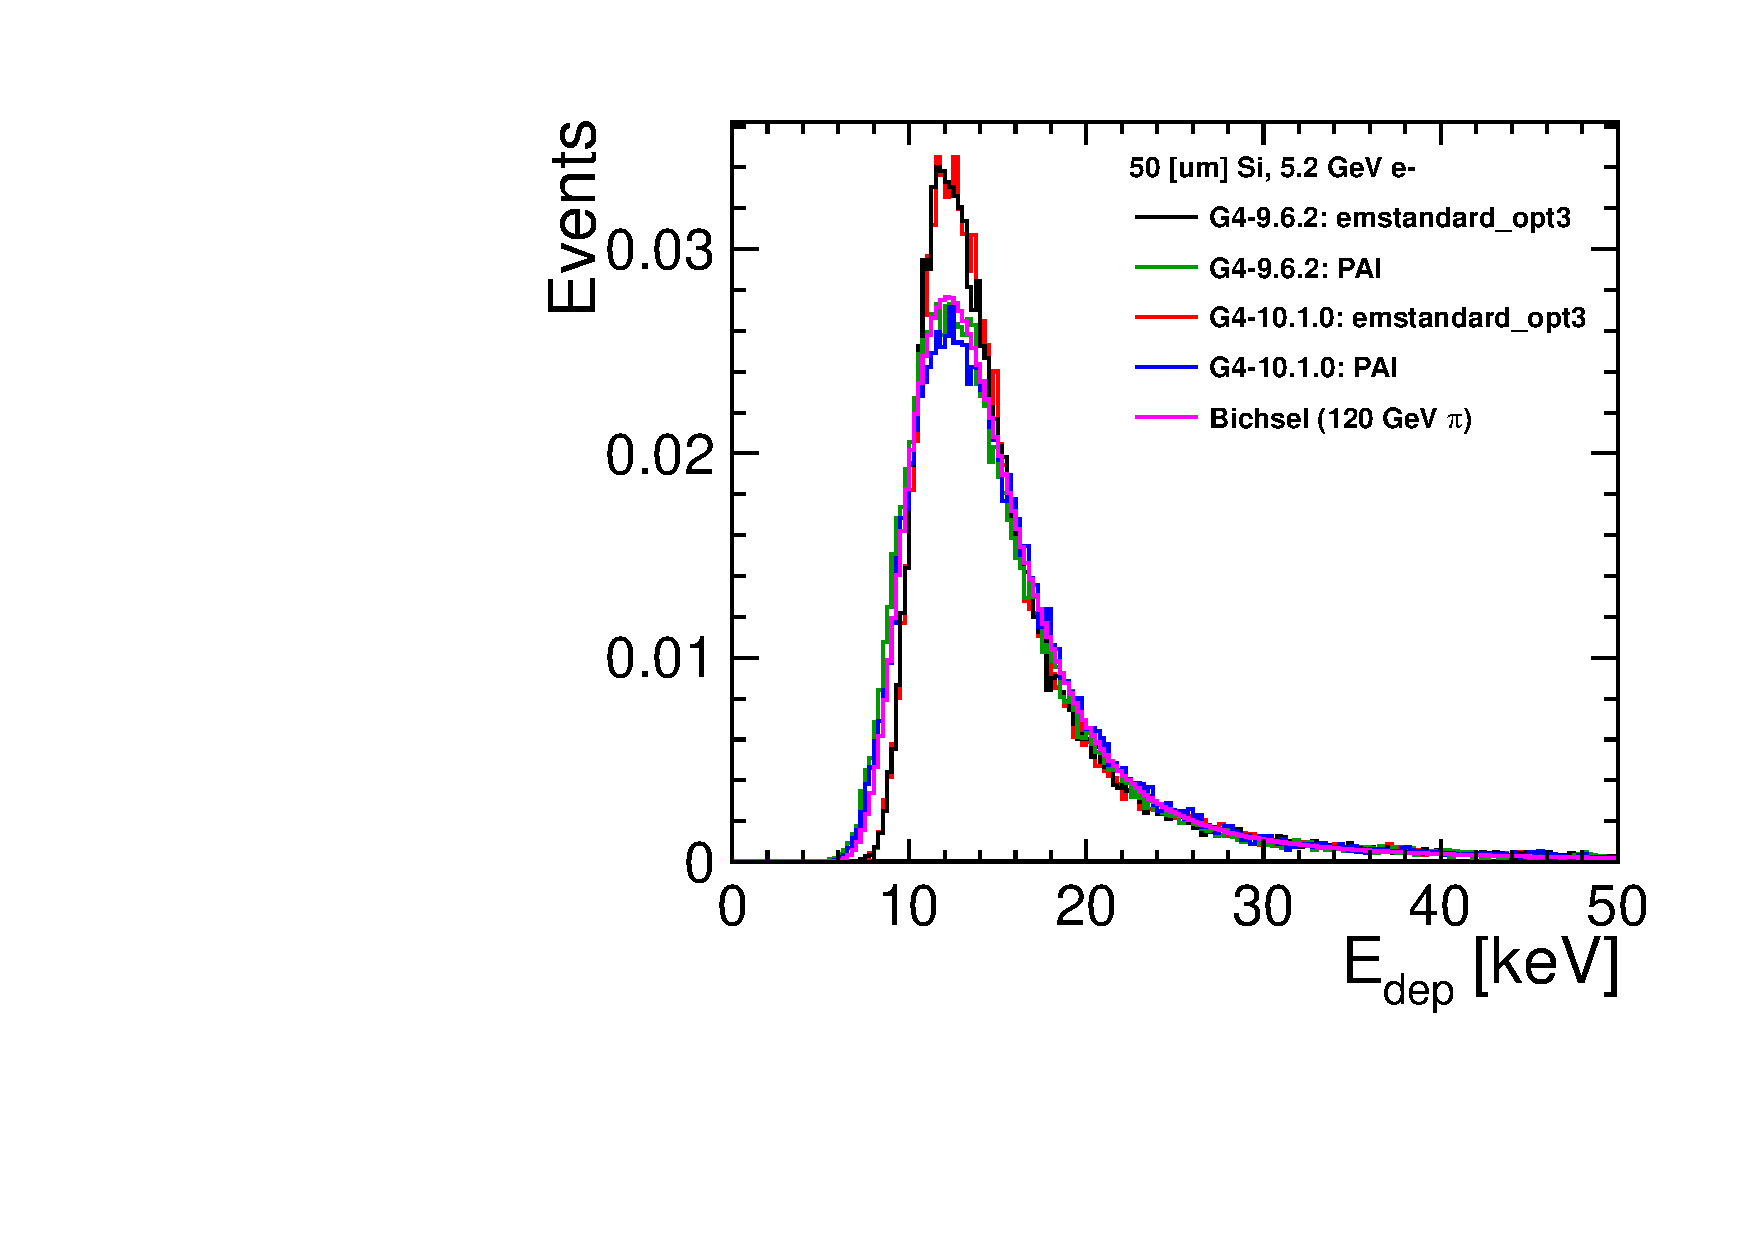
\includegraphics[width=0.5\textwidth]{figures/50um_bichsel_physicsLists.pdf}
  \caption{Energy-loss distribution in $50\,\micron$ silicon comparing
    the Bichsel model and different physics list in \textsc{Geant4}.}
  \label{fig:BichselVSG4}
\end{figure}

%% --------------------------------------------- %%
\section{Transport of charge carriers in silicon}

In silicon detectors, the movement of the charge carriers (holes and
electrons) lead to signal pulses in the electrical contacts which can
be detected by the readout electronics. 
In absence of any external electric field, free charge carriers move
randomly and are scattered due to their collisions to the crystal
lattice or other impurities. In average, in equilibrium conditions,
the traveled distance averaged over charges is zero. In addition to
the statistical movement, two other mechanisms can affect the
transport of charge carriers: diffusion (due to a gradient in
concentration) and drift (in the presence of an external electric
field).

The diffusion implies that a carrier is more probable to move from a
high-concentration region to a low-concentration region. The diffusion
current per unit area is given by Equation~\ref{eq:diffusionCurrent}~\cite{Rossi:976471}:

\begin{equation}
  \begin{aligned}
    J_{n, diff}=-{kT \over e} \mu_n \nabla n \qquad \textnormal{for electrons}
    \; , \\
    J_{p, diff}={kT \over e} \mu_p \nabla p \qquad \textnormal{for holes}
    \; , 
  \end{aligned}
  \label{eq:diffusionCurrent}
\end{equation}
where $k$ is the Boltzmann constant, $T$ the absolute temperature, $e$ the
elementary charge, $\mu$ the mobility of the charge carriers, $\nabla
n$ and $\nabla p$ are the gradients of the electron and hole
concentrations.

Charge carriers are accelerated between two random collisions in the
presence of an external electric field in the direction of the field
and leads to and average drift velocity given by
Equation~\ref{eq:driftVelocity}~\cite{Rossi:976471}:

\begin{equation}
  \begin{aligned}
    v_{n}=-\mu_n \textbf{E} \qquad \textnormal{for electrons}
    \; , \\
    v_{p}=\mu_p \textbf{E} \qquad \textnormal{for holes}
    \; , 
  \end{aligned}
  \label{eq:driftVelocity}
\end{equation}
where $v$ is the average drift velocity, $\textbf{E}$ the electric
field and $\mu$ the mobility of the charge carriers. The mobility is a
function of the electric field. For higher electric fields the charge
carriers gain more acceleration and the number of collisions per unit
time becomes highe. This leads to a saturation of the drift velocity
$v_s$. The mobility dependence on the electric field is described by
Equation~\ref{eq:mobility} and parameters described in
Table~\ref{tab:mobility_parameters}~\cite{Jacoboni197777}:
\begin{equation}
  \mu=\frac{v_{s}/E_{c}}{\left[1+(E/E_{c})^{\beta}\right]^{1/\beta}}\; .
  \label{eq:mobility}
\end{equation}

\begin{table}[htbp]
  \centering
  \caption{Parameters for the mobility as described in
    Equation~\ref{eq:mobility} with T the absolute temperature and E
    the absolute electric field.}
  \label{tab:mobility_parameters}
  \begin{tabular}{c c c c}
    \toprule
    Parameter & Electrons & Holes & unit \\
    \midrule
    $v_s$ & 1.53 $\times$ $10^9$ $\times$ T\textsuperscript{-0.87} &
1.62 $\times$ $10^8$ $\times$ T\textsuperscript{-0.52} & cm/s \\ 
    $E_c$ & 1.01 $\times$ T\textsuperscript{1.55} & 1.24 $\times$ T\textsuperscript{1.68} & V/cm \\ 
    $\beta$ & 2.57 $\times$ $10^{-2}$ $\times$ T\textsuperscript{0.66} & 0.46 $\times$ T\textsuperscript{0.17} & -\\
    \bottomrule
  \end{tabular}
\end{table}

Figure~\ref{fig:Mobility_electron_holes} shows the mobility for
electrons and holes as a function of the electric field. For a low electric field, the mobility for intrinsic silicon at 300~K
is:
\begin{equation*}
  \begin{aligned}
    \mu_n=1415 \pm 46 \qquad \textnormal{\cmsquared/(Vs)} \; , \\
    \mu_p=480 \pm 17 \qquad \textnormal{\cmsquared/(Vs)} \; .
  \end{aligned}
\end{equation*}

Holes are three times less mobile than electrons which make them more
likely to be trapped in an irradiated material.

\begin{figure}[htbp]
  \centering
  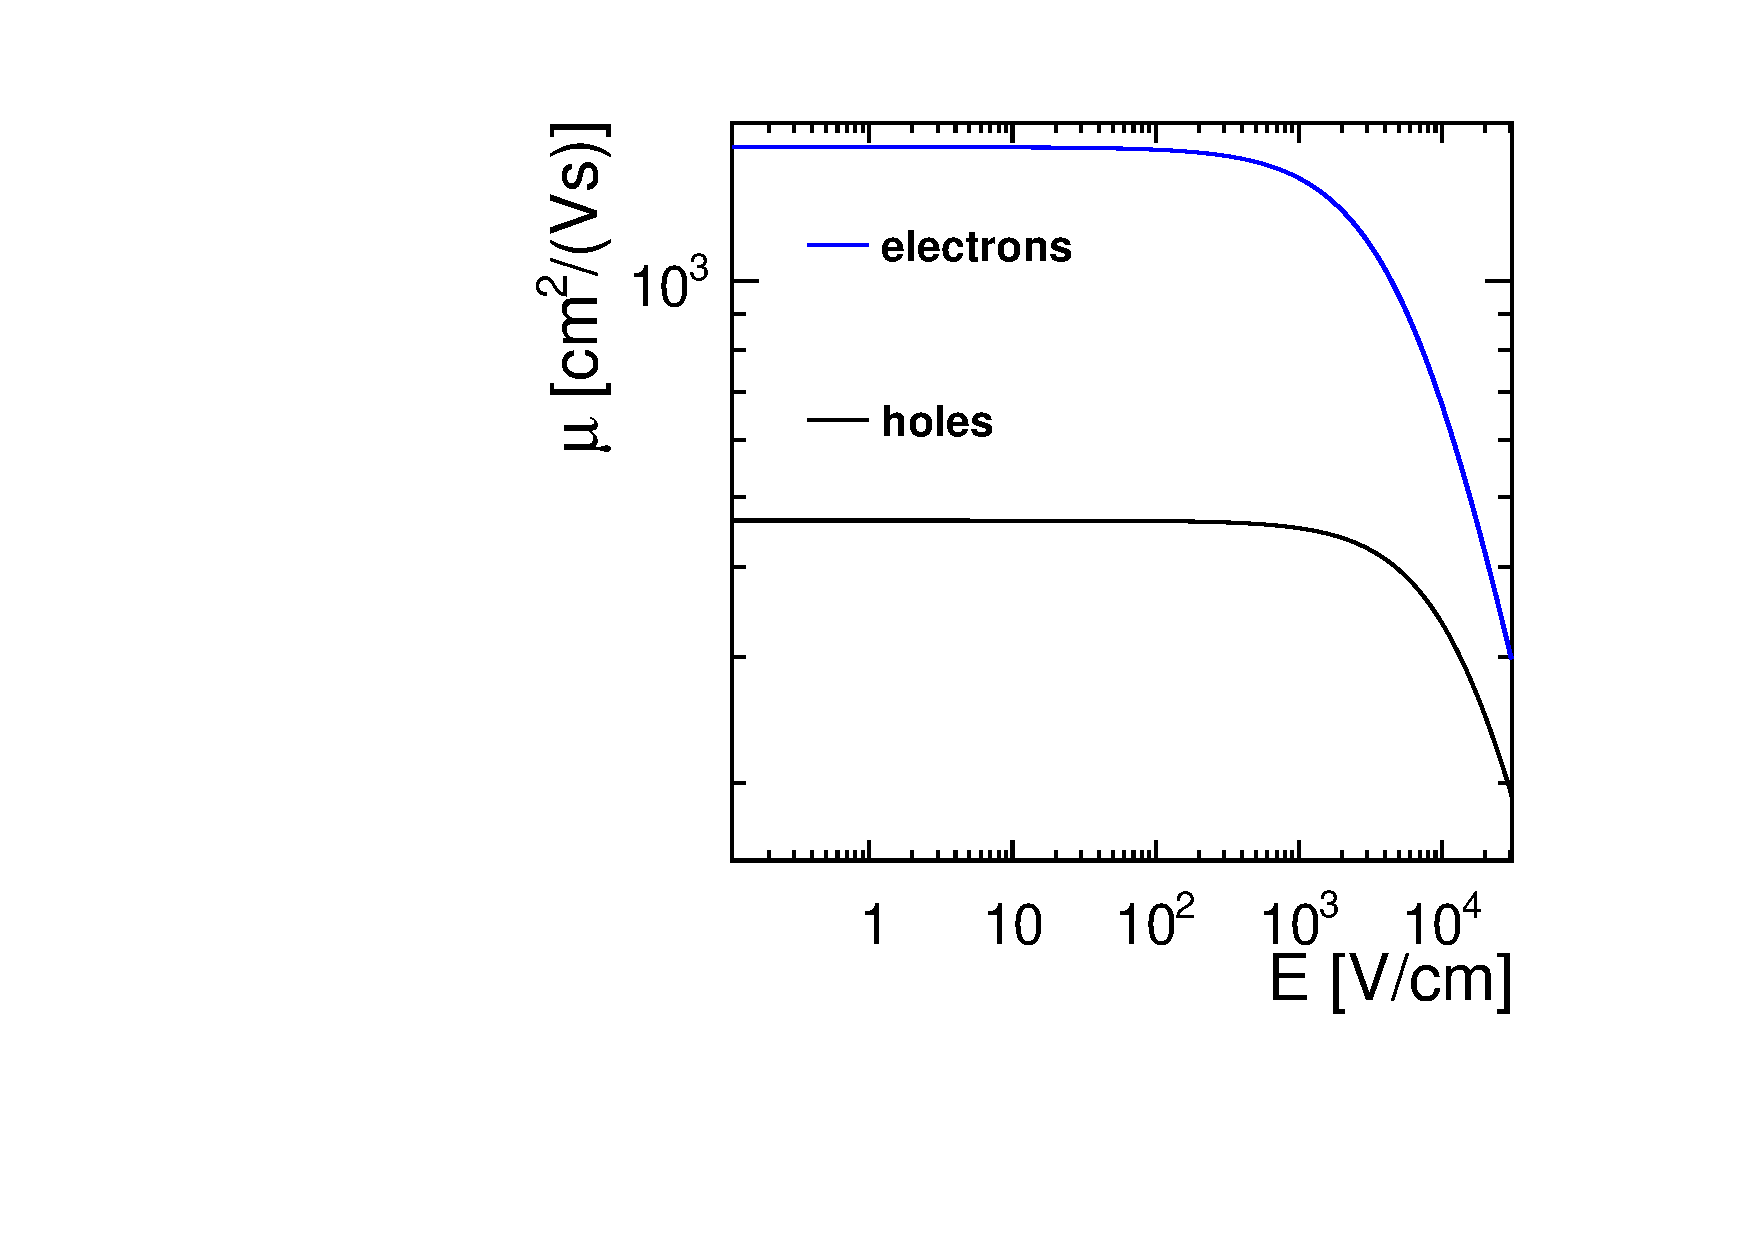
\includegraphics[width=0.5\textwidth]{figures/ChargeSharing/Mobility_electron_holes.pdf}
  \caption{Mobility for electrons and holes as a function of an
    applied electric field calculated with the Equation~\ref{eq:mobility}.}
  \label{fig:Mobility_electron_holes}
\end{figure}
%% --------------------------------------------- %%
\section{Pixel detectors: pn-junction}
The potential $\varphi$ at each point is described by Poisson's equation~\ref{eq:poisson} \cite{Knoll2010}
\begin{equation}
  \nabla^{2}  \varphi=-{\rho \over \epsilon}\; ,
  \label{eq:poisson}
\end{equation}

where $\epsilon$ is the dielectric constant of the medium and $\rho$ the net charge density.
The electric field E due to the electric potential is obtained by Equation~\ref{eq:Efield}

\begin{equation}
E=-grad \varphi \; ,
\label{eq:Efield}
\end{equation}

In one dimension, Equation~\ref{eq:poisson} becomes
\begin{equation}
{{d^{2}  \varphi(z)} \over {dz^{2}}}=-{\rho(z) \over \epsilon}\; ,
\label{eq:poisson1D}
\end{equation}

To simplify, we assume an abrupt junction where the charge densities on the p and n sides are:
\begin{equation}
  \rho(z)= 
  \begin{cases} 
    eN_{D}, & \mbox{if } 0\leq z < z_{n}\\ 
    -eN_{A}, & \mbox{if } z_{p}\leq z < 0 
  \end{cases} 
  \; ,
\label{eq:chargeDensity}
\end{equation}

First, considering the n-side, the first and second integrations of the Poisson equation give,
\begin{equation}
    {{d\phi(z)} \over {dz}}=-{{eN_{d}} \over \epsilon} (z-z_{n}) 
    \; ,
    \label{eq:PoissonIntegration1}
  \end{equation}

\begin{equation}
  \phi(z)=-{{eN_{d}} \over \epsilon} {z^{2} \over 2}+{{eN_{d}zz_{n}}\over \epsilon}+Vj
  \; ,
  \label{eq:PoissonIntegration2}
\end{equation}

Where $V_j$ is the potential at the interface where the n- and the p-sides join. At the boundary of the depletion region $z=z_{n}$:

\begin{equation}
  \phi(z_{n})=V_{b}={{eN_{d}z_{n}^{2}} \over \epsilon}+V_j 
  \; ,
  \label{eq:BounderyPotential}
\end{equation}

In the p-region,
\begin{equation}
  V_j={{eN_ax_p^2} \over {2\epsilon}}
  \; ,
\end{equation}

And the total potential,
\begin{equation}
V_b={{e} \over {2 \epsilon}}(N_dx_n^2+N_ax_p^2)
  \; ,
\end{equation}

The overall charge neutrality is maintained,
\begin{equation}
N_d x_n=N_a x_p
  \; ,
\end{equation},

the reverse bias potential can be expressed as

\begin{equation}
V_b={e \over {2\epsilon}}\left(1+{N_a \over N_d}\right) N_a x_p^2={e \over {2\epsilon}}\left(1+{N_d \over N_a}\right) N_d x_n^2
  \; .
\end{equation}

The depletion widths on the n- and p-sides of the junction are

\begin{equation}
  \begin{multlined}
x_n=\sqrt{{2 \epsilon V_b} \over {eN_d(1+N_d/N_a)}} \\
x_p=\sqrt{{2 \epsilon V_b} \over {eN_a(1+N_a/N_d)}} 
\; ,
\end{multlined}
\end{equation}

The total depletion width is 

\begin{equation}
W=x_n+x_p=\sqrt{{2 \epsilon V_b \left(N_a+N_d\right)} \over {eN_aN_d} }
\; ,
\end{equation}

The junction potential and also for an asymmetrical junction with $N_d \ll N_a$ for which the junction potential is equal to the potential of the p-contact.

\begin{equation}
V_j=\left(N_d \over N_a\right) {V_b \over \left(  1+N_d/N_a \right)} \stackrel{N_d \ll N_a}{\approx} {N_d \over N_a}V_b
\; ,
\end{equation}


For a pixel detector with asymmetric junction with a highly doped surface $N_c$ concentration and a lightly doped bulk $N_b$ ($N_b \ll N_c$), the doping concentration is expressed in terms of resistivity 
\begin{equation}
\rho_b = {1 \over {e\mu_{b}N_{b}}}
\; ,
\end{equation}
where $\mu_b$ and $N_b$ are the mobility and the doping concentration of the bulk. The depletion width $W$ becomes,
\begin{equation}
W=\sqrt{2 \epsilon \mu_b \rho_bV_b}
\; ,
\label{eq:depletionWidth}
\end{equation}

In the absence of an externally applied voltage to a pn-junction, the thermal diffusion of the electrons and the holes from their original atoms results in a depletion width with a potential difference between the p- and n-sides called the built-in potential $V_{bi}$ which is about 0.5~V for detector diodes. \\
By taking into account the built-in reverse bias voltage, Equation~\ref{eq:depletionWidth} is written as,
\begin{equation}
W=\sqrt{2 \epsilon \mu_b \rho_b \left(V_b+V_{bi}\right)}=\sqrt{{2 \epsilon \left(V_b+V_{bi}\right)} \over {eN_b}}
\; ,
\label{eq:depletionWidth2}
\end{equation}

The electric field of Equation~\ref{eq:PoissonIntegration1}, by replacing the depletion width and $N_d$ by Equation~\ref{eq:depletionWidth2} can be expressed as
\begin{equation}
E(z)={{2\left(V_b+V_{bi}\right)} \over {W}} \left({z \over W}-1\right)
\; ,
\end{equation}

The depletion voltage ($W=d$) can be expressed as,
\begin{equation}
V_D={{eN_bd^2} \over {2 \epsilon}}-V_{bi}
\; ,
\label{eq:depletionVoltage}
\end{equation}
where $d$ is the detector thickness. \\

The electric field drops linearly from its maximum value at the junction to zero at the opposite contact. Increasing the bias voltage beyond the needed bias to completely deplete the detector adds a uniform field. By neglecting the built-in voltage (as the bias voltage is much higher than that), the electric field is written as,
\begin{equation}
E(z)={{V_B-V_D} \over d}+\left(1-{z \over d}\right)2{V_D \over d}
\; ,
\label{eq:Efield}
\end{equation}

The charge carriers, drift through the silicon detector with a velocity as defined by,

\begin{equation}
  \vec{v}_{drift}=\mu_c \cdot \vec{E}\; ,
\end{equation}

In one-dimension, and considering $\mu_c$ constant, the drift velocity is written as
\begin{equation}
v_{drift}={{dz} \over {dt}}=\mu_c \cdot E(z)
\; ,
\end{equation}

The time required for a charge originating at point $z_0$ to reach a point $z$ is
\begin{equation} 
  t(z)=\int_{z_0}^{z} {{ds} \over {\mu_c \cdot E(s)}}
  \; ,
  \label{eq:driftTimeIntegral}
\end{equation}

By integrating Equation~\ref{eq:driftTimeIntegral} and replacing the electric field by Equation~\ref{eq:Efield} one obtains:

\begin{equation} 
  t(z, z_0)={{d^2} \over {2 \mu_c V_D}} ln\left( {{d(V_B+V_D)-2V_Dz_0} \over {d(V_B+V_D)-2V_Dz}} \right)
  \; ,
  \label{eq:driftTimeIntegratedz0}
\end{equation}

In Equation~\ref{eq:driftTimeIntegratedz0}, by replacing $z_0=0$, we obtain:
\begin{equation} 
  t(z)={{d^2} \over {2 \mu_c V_D}} ln\left( {{V_B+V_D} \over {V_B+V_D-2V_Dz/d}} \right)
  \; ,
  \label{eq:driftTimeIntegrated}
\end{equation}

And the diffusion sigma is given by,

\begin{equation} 
  \sigma_{diffusion}\left(z\right)=\sqrt{2 D_{b} t_{c}}=\sqrt{{{kTd^2}\over{eV_D}}ln\left({{V_B+V_D}\over{V_B+V_D-2V_Dz/d}}\right)}
  \; ,
  \label{eq:driftTimeIntegrated}
\end{equation}


\begin{table}[htpb]
  \centering
  \caption{Sensors characteristics:}
  \label{tab:Efield_mobility}
  \begin{tabular}{ c c c c c c }
    \toprule
    Assembly & Sensor type & Thickness & V\textsubscript{depletion} &  V\textsubscript{bias} & THL\textsubscript{op} \\
    \midrule
    A06-W0110 & p-in-n & 50~\micron & $<15$~V & 15~V & 326 (855e\textsuperscript{-}) \\
    L04-W0125 & p-in-n & 100~\micron & 19.64~V & 35~V & 410 (916e\textsuperscript{-}) \\
    B06-W0125 & n-in-p & 200~\micron  & 30.31~V & -50~V & 435 (1066e\textsuperscript{-}) \\
    \bottomrule
  \end{tabular}
\end{table}

\begin{figure}[htbp]
  \centering
  \begin{subfigure}[b]{0.33\textwidth}
    \centering
    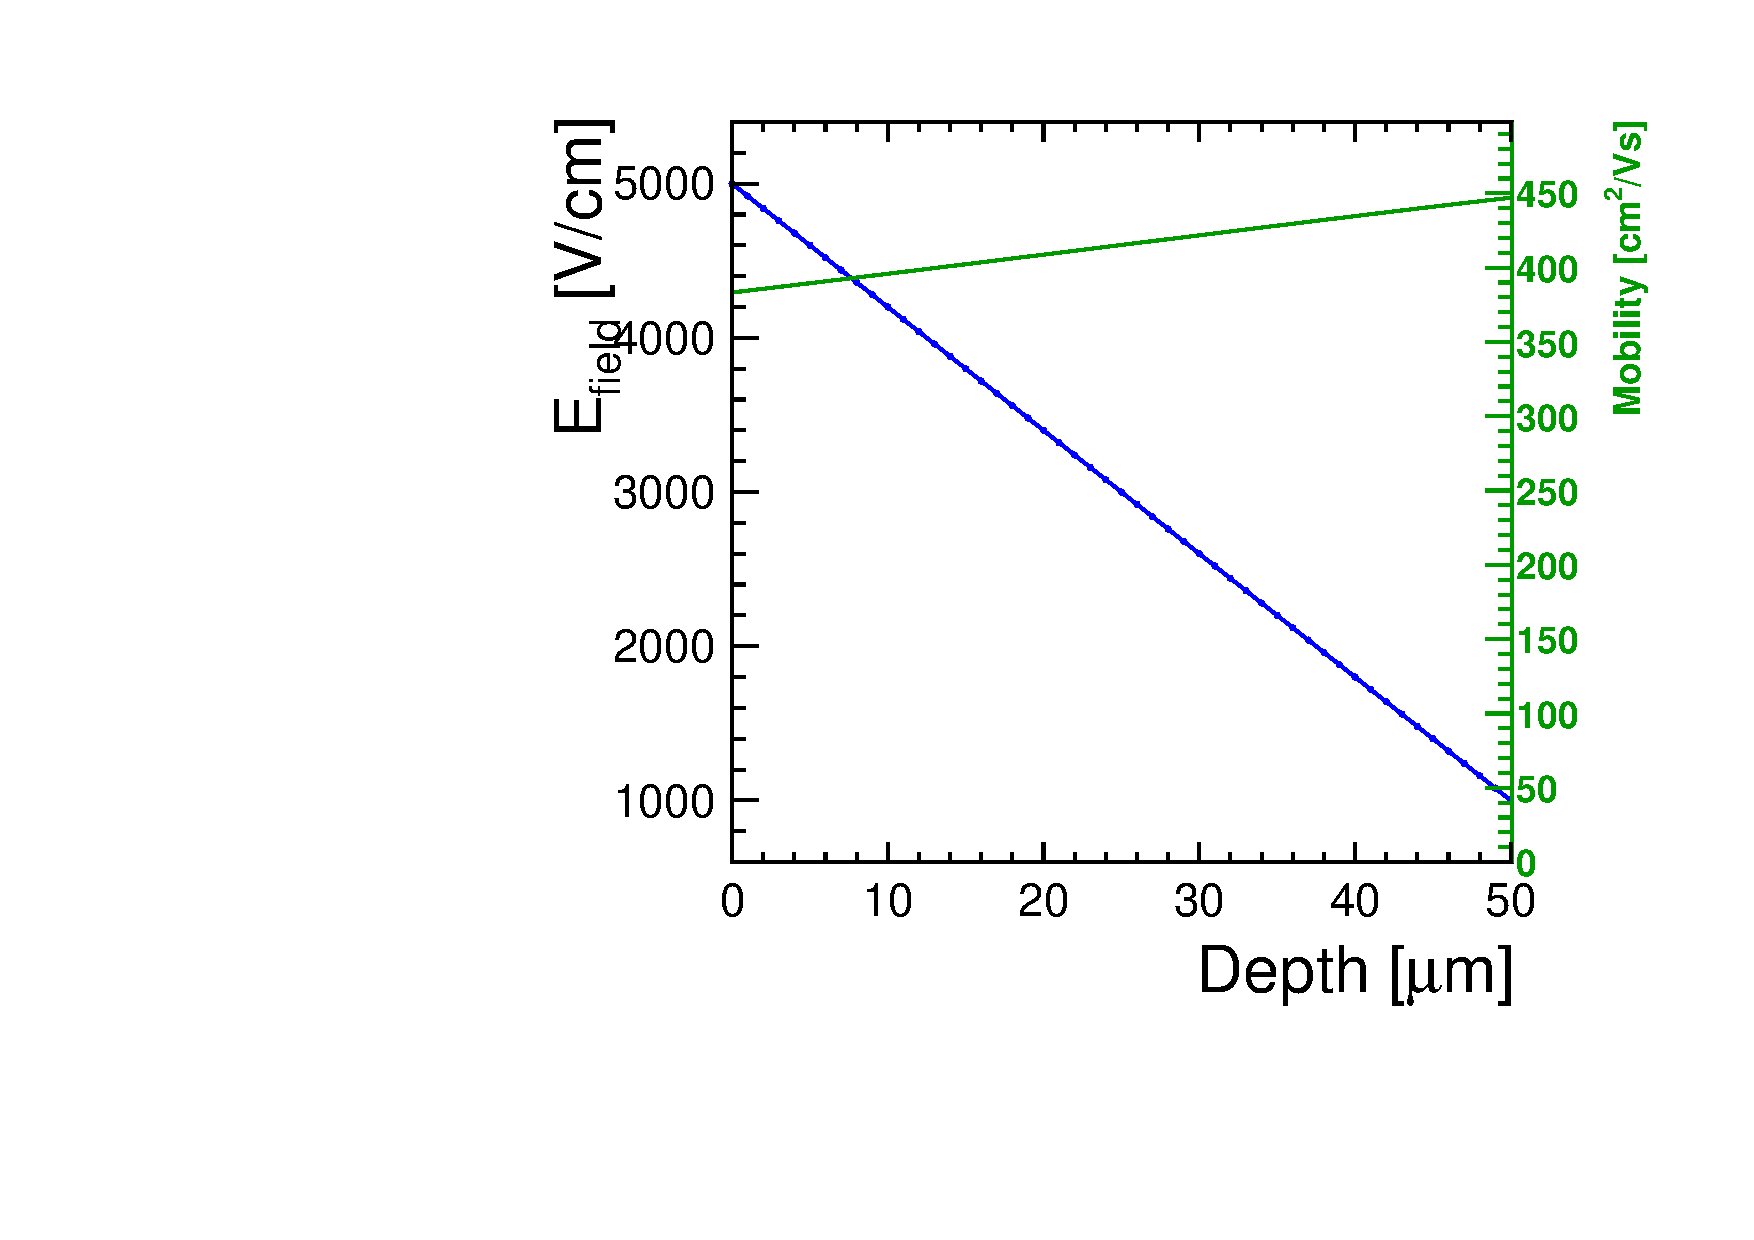
\includegraphics[width=\textwidth]{figures/ChargeSharing/Efield_mob_A06.pdf}
    \caption{50~\micron silicon}\label{fig:Mob_Efield_A06}
  \end{subfigure}\hfill
  \begin{subfigure}[b]{0.33\textwidth}
    \centering
    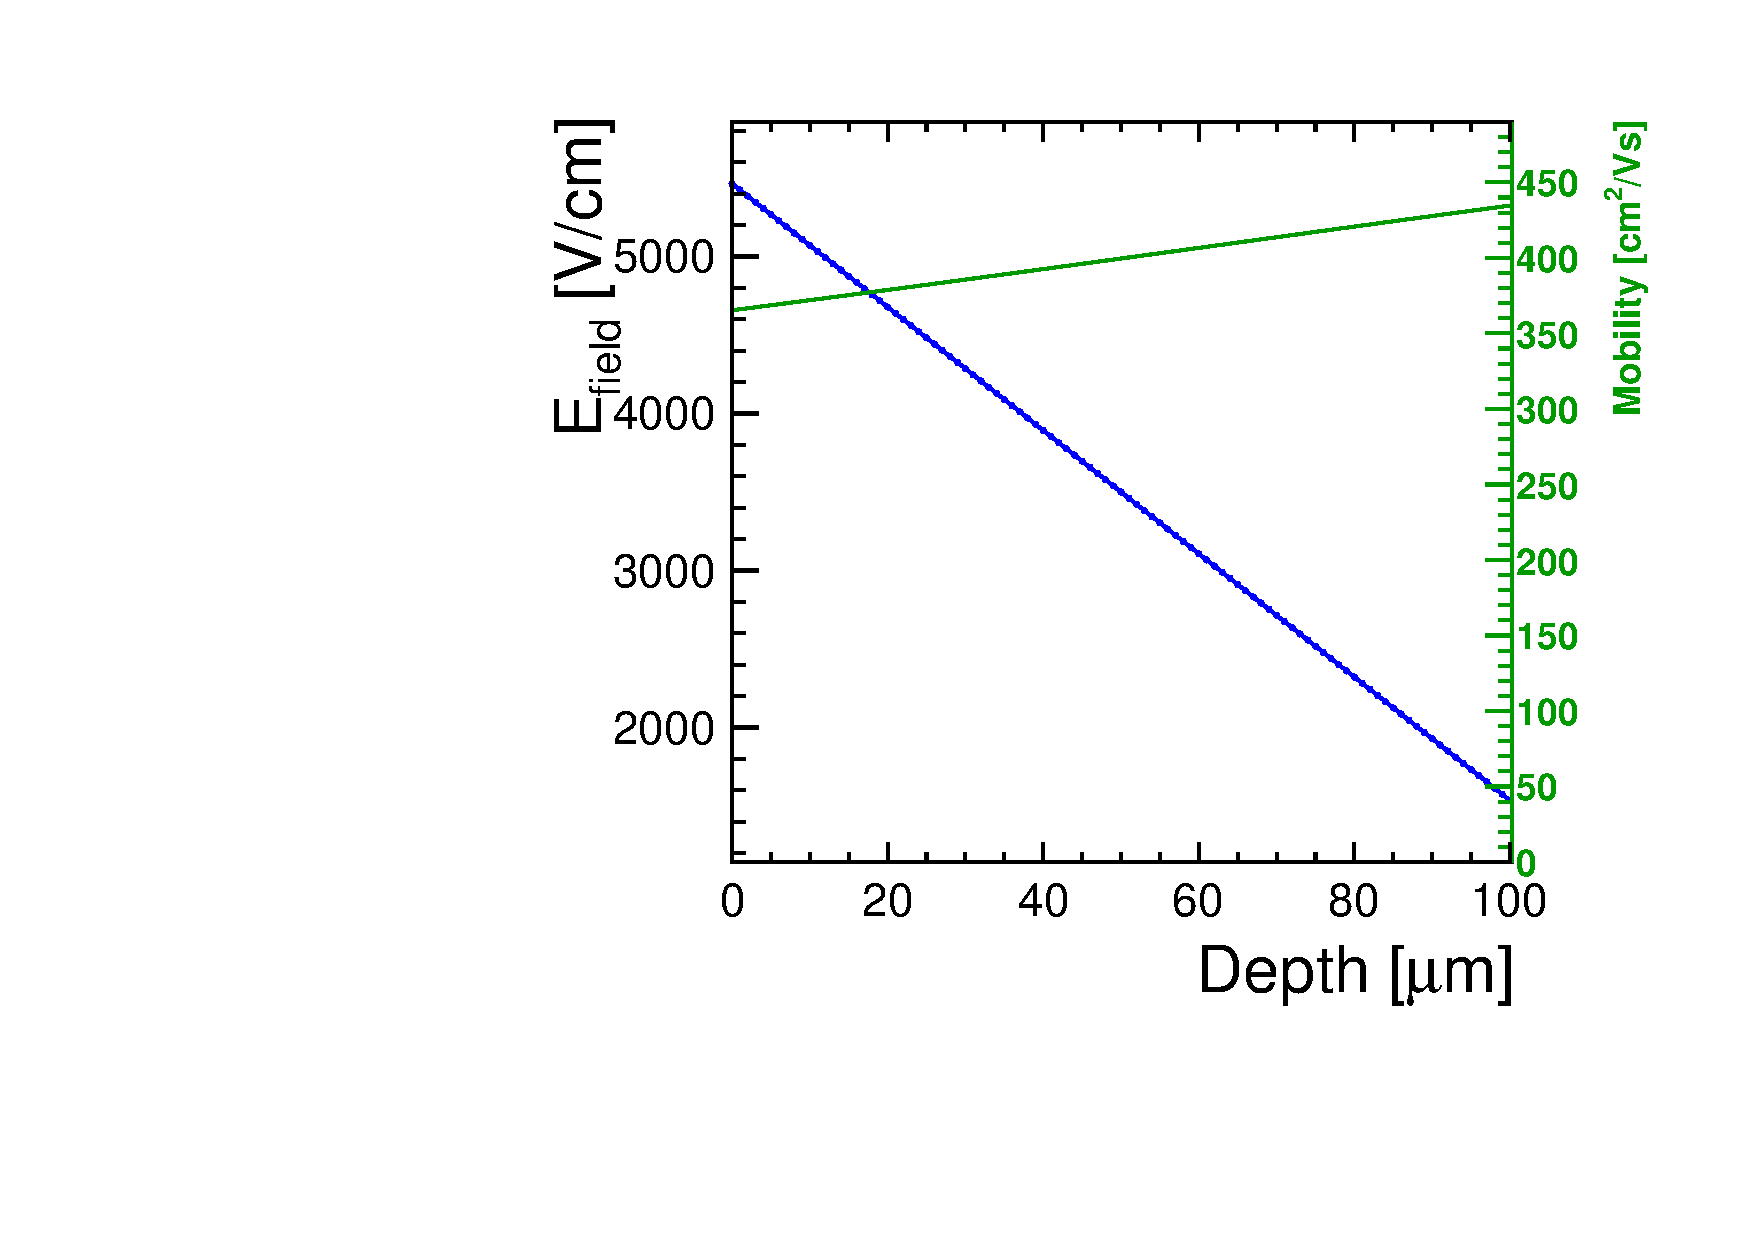
\includegraphics[width=\textwidth]{figures/ChargeSharing/Efield_mob_L04.pdf}
    \caption{100~\micron Silicon}\label{fig:Mob_Efield_L04}
  \end{subfigure} \hfill
  \begin{subfigure}[b]{0.33\textwidth}
    \centering
    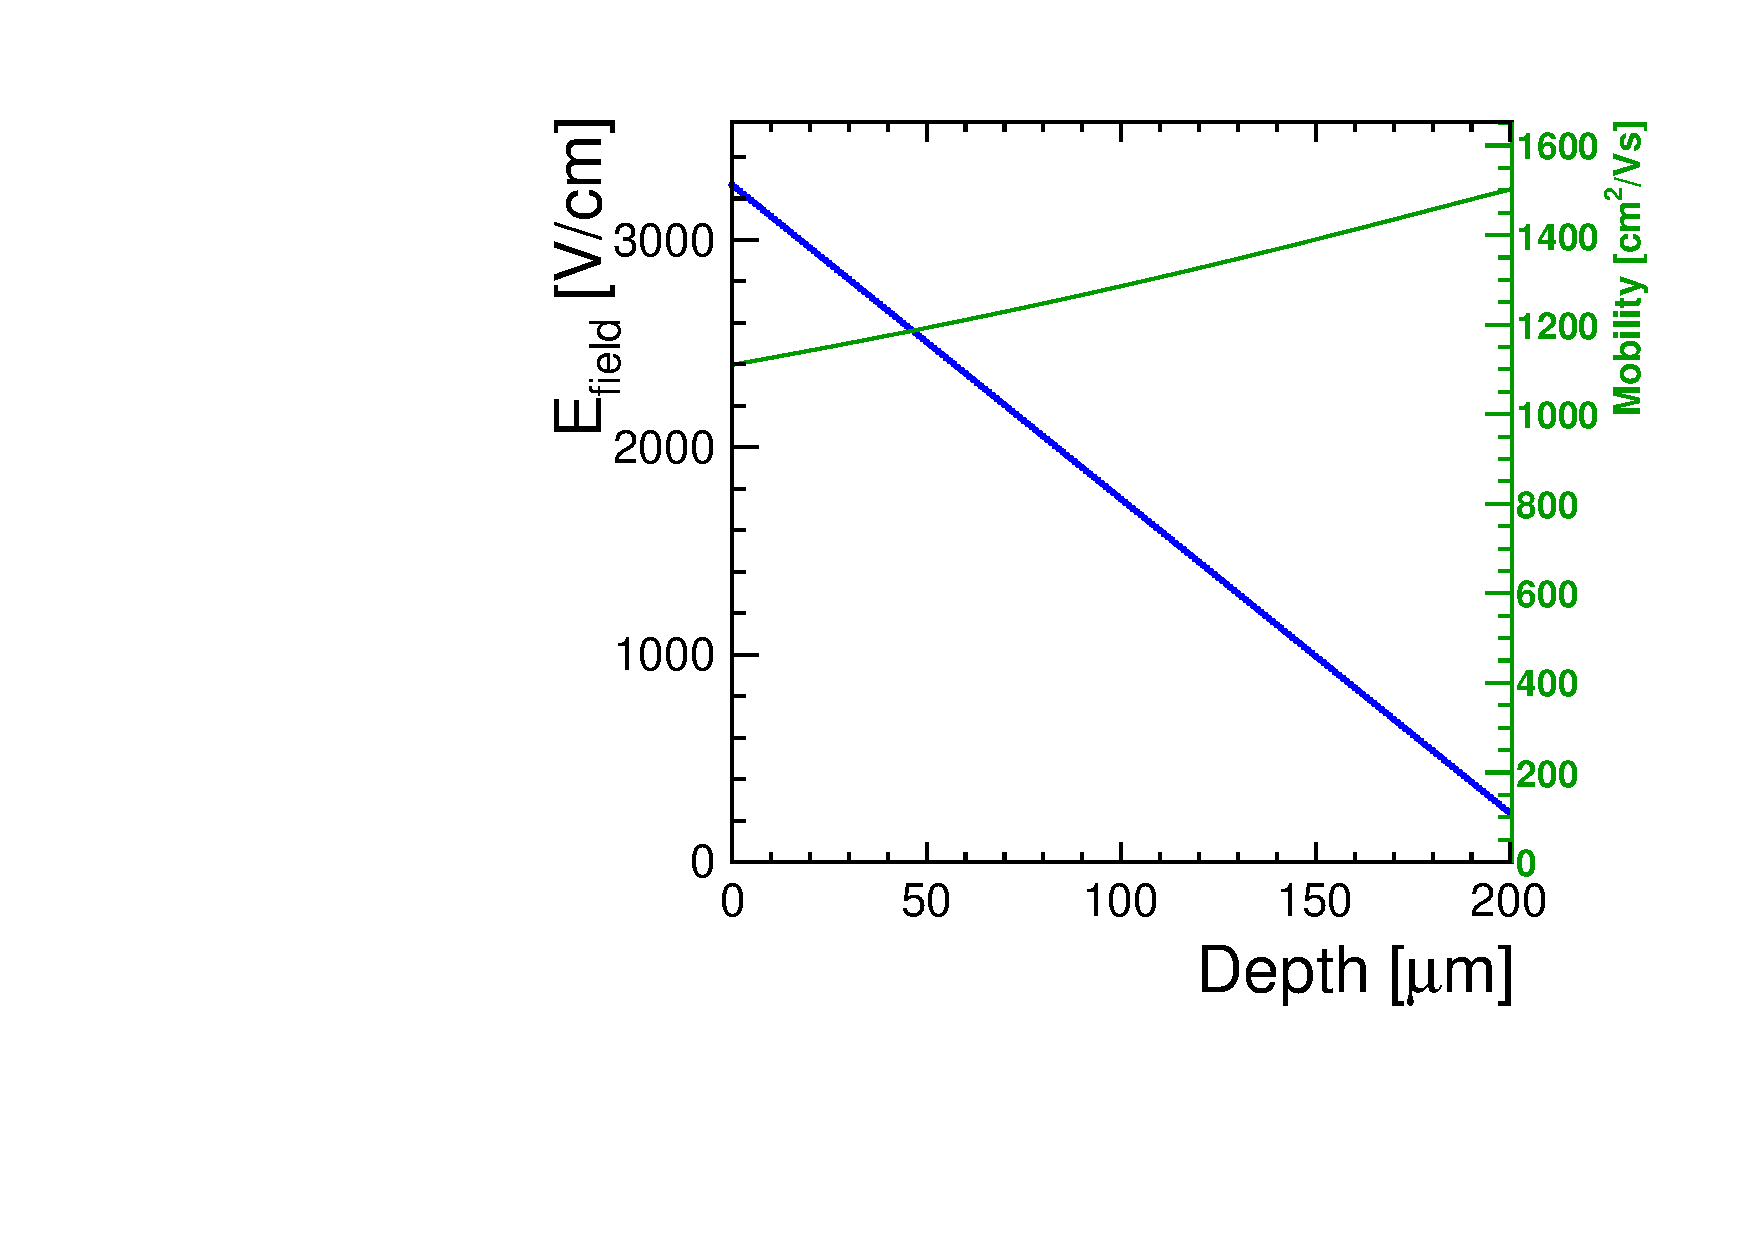
\includegraphics[width=\textwidth]{figures/ChargeSharing/Efield_mob_B06.pdf}
    \caption{200~\micron Silicon}\label{fig:Mob_Efield_B06}
  \end{subfigure} 
  \caption{Mobility dependence on the electric field.}\label{fig:Efield_mobility}
\end{figure}

Assuming the mobility constant is a good approximation for calculating
the charge sharing spread since the electric field is low. An example
is given for the case where the silicon sensor has a thickness of 200~\micron.

\begin{figure}[htbp]
  \centering
  \begin{subfigure}[b]{0.49\textwidth}
    \centering
    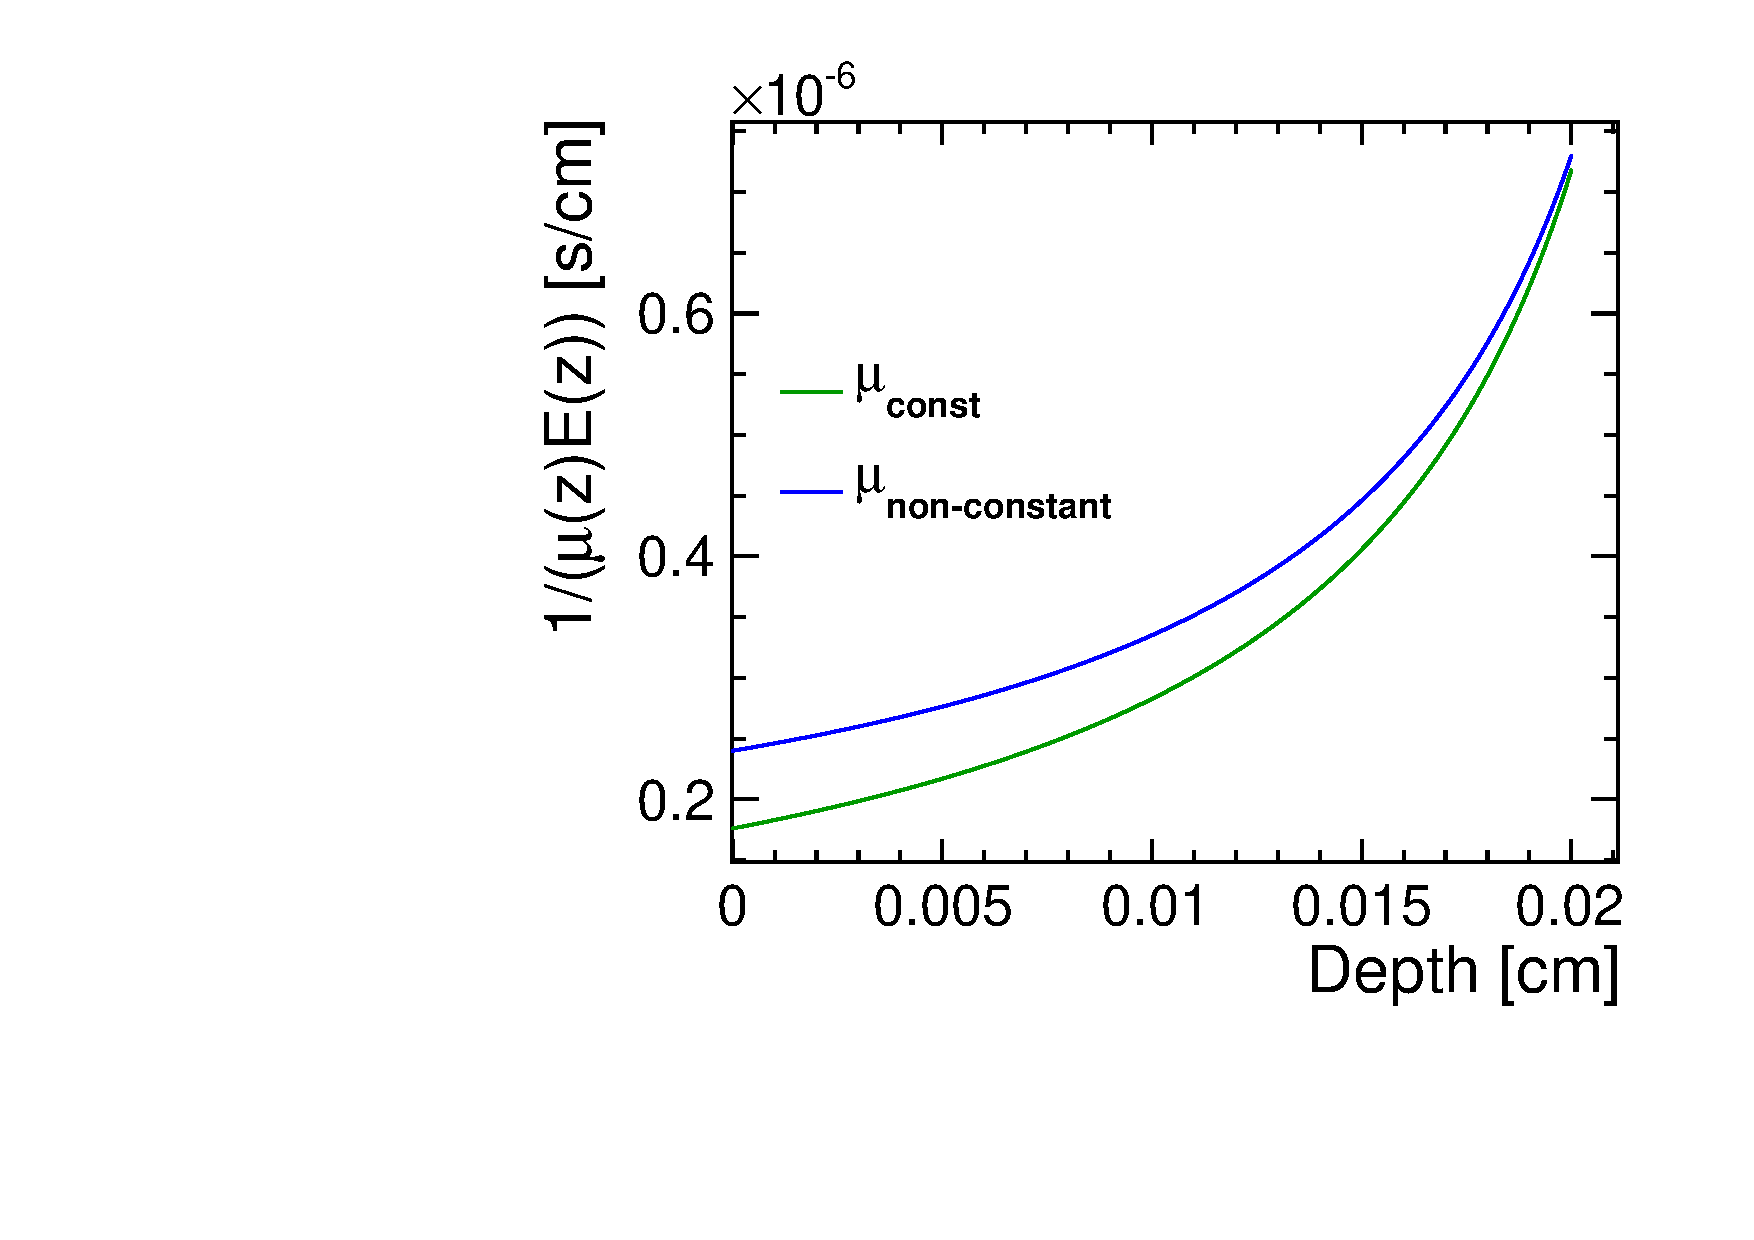
\includegraphics[width=\textwidth]{figures/ChargeSharing/B06_FunctionToIntegrate.pdf}
    \caption{}\label{fig:}
  \end{subfigure}\hfill
  \begin{subfigure}[b]{0.49\textwidth}
    \centering
    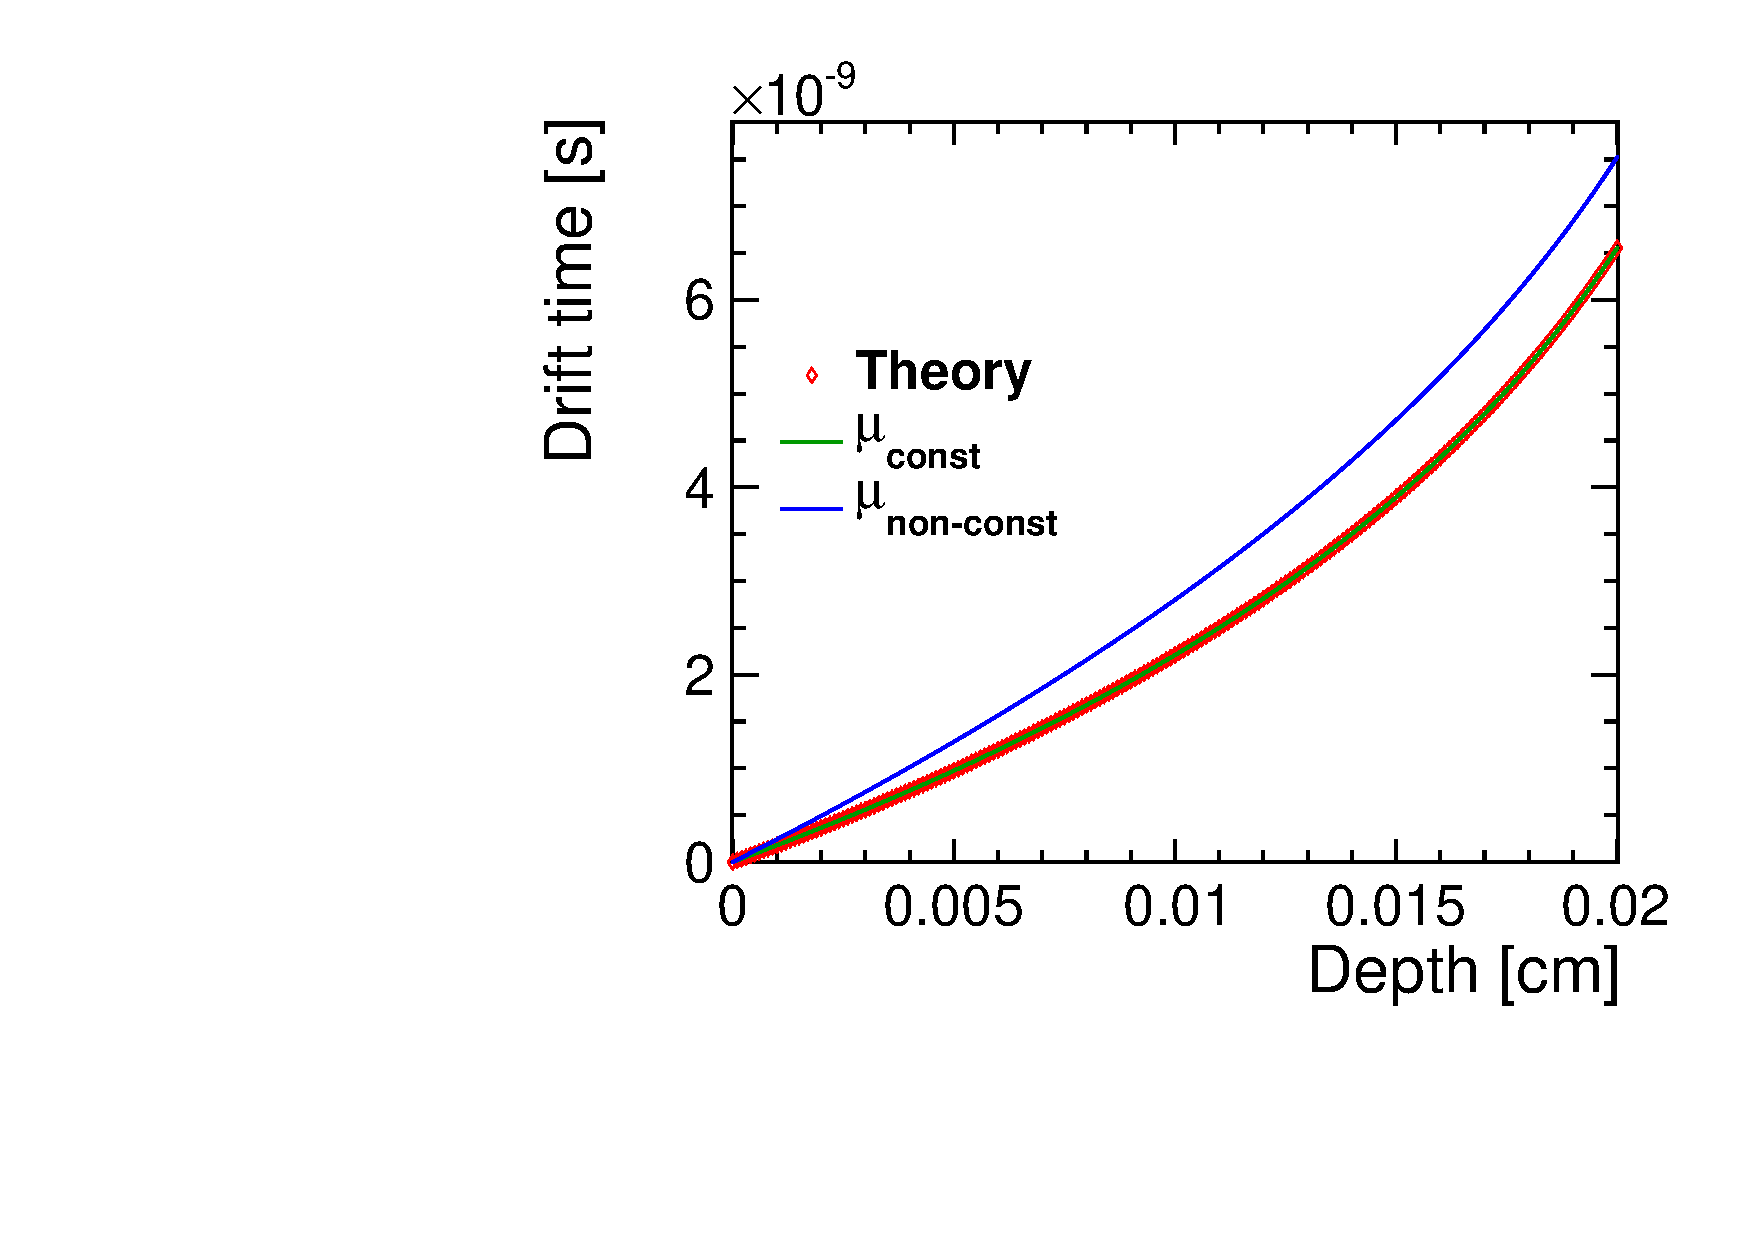
\includegraphics[width=\textwidth]{figures/ChargeSharing/B06_driftTime.pdf}
    \caption{}\label{fig:}
  \end{subfigure} 
  \caption{Drift time considering the mobility constant or non-constant.}\label{fig:}
\end{figure}

The diffusion constant and the diffusion spread considering the
mobility constant and non-constant.
\begin{figure}[htbp]
  \centering
  \begin{subfigure}[b]{0.49\textwidth}
    \centering
    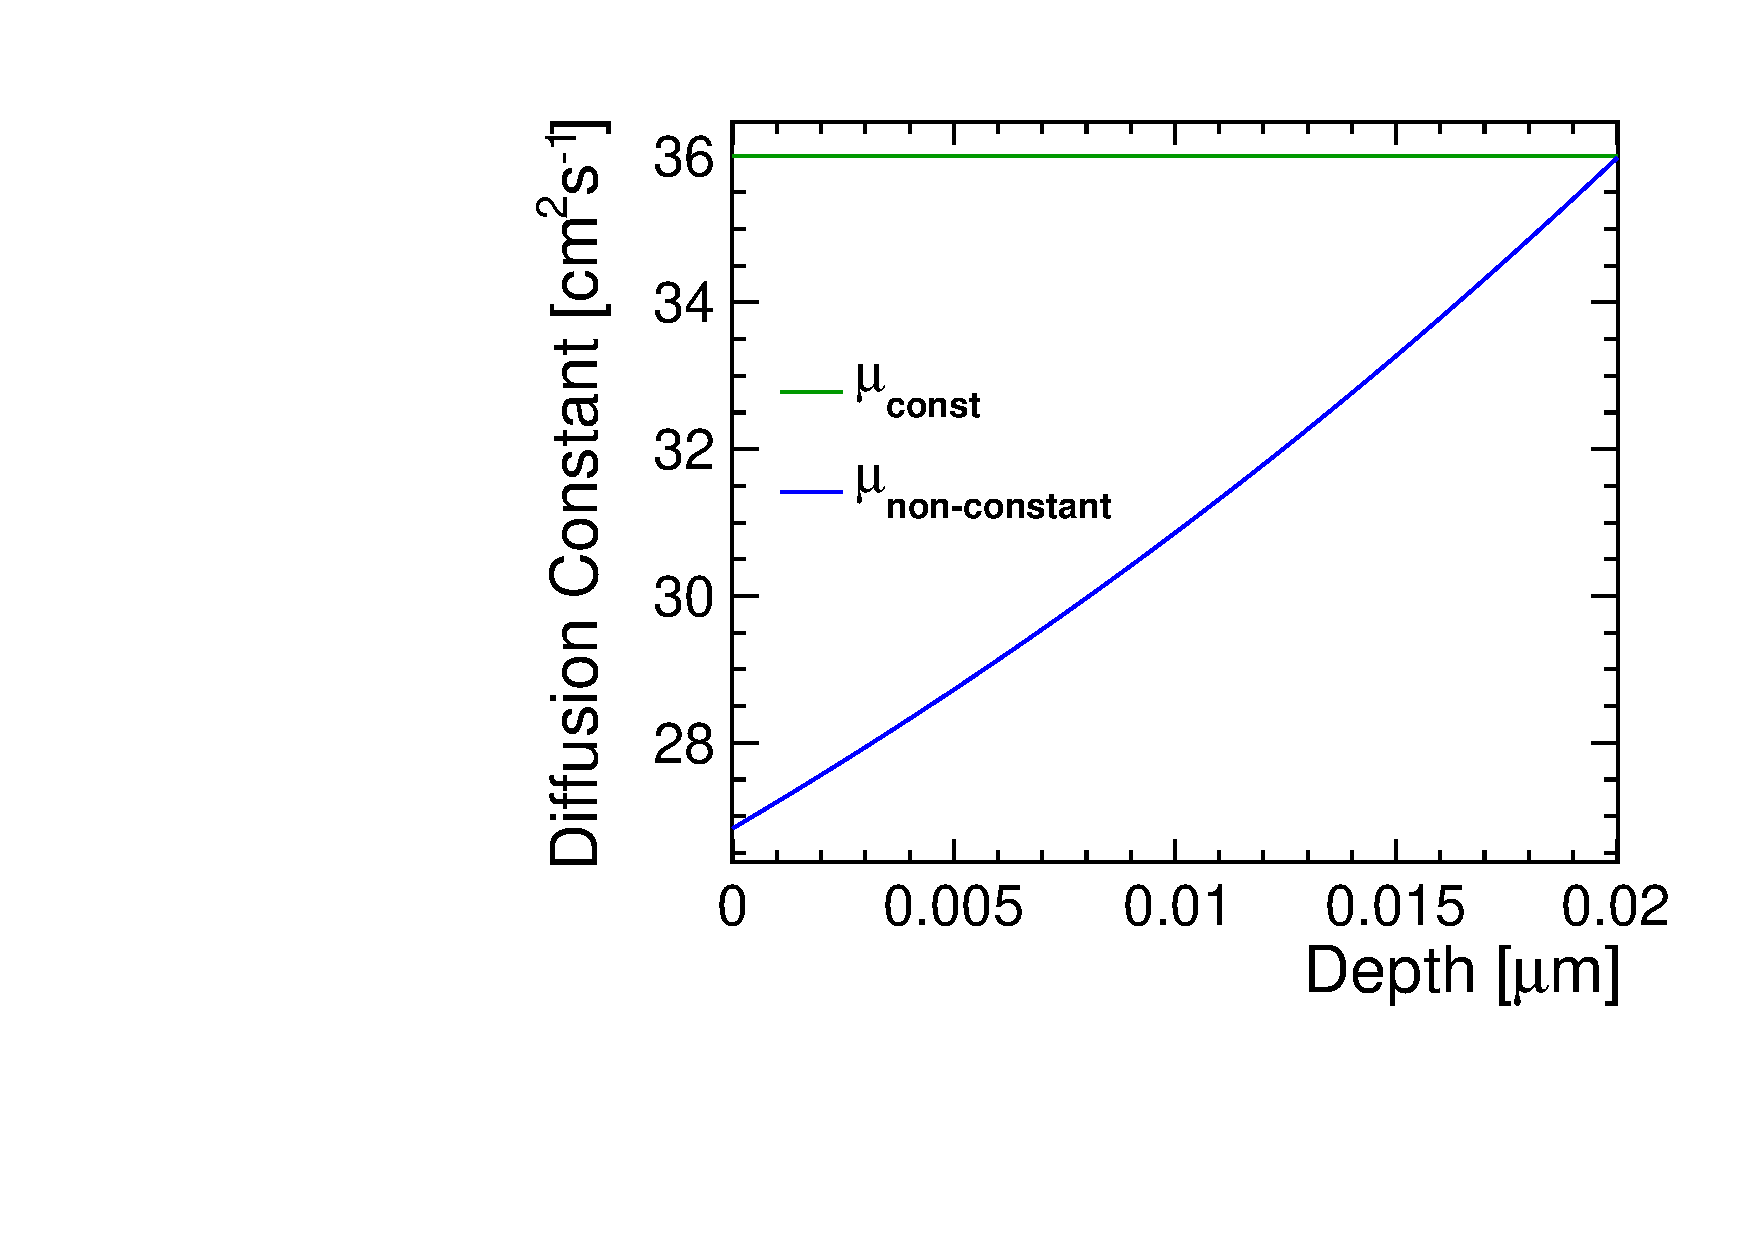
\includegraphics[width=\textwidth]{figures/ChargeSharing/B06_DiffusionConstant.pdf}
    \caption{}\label{fig:}
  \end{subfigure}\hfill
  \begin{subfigure}[b]{0.49\textwidth}
    \centering
    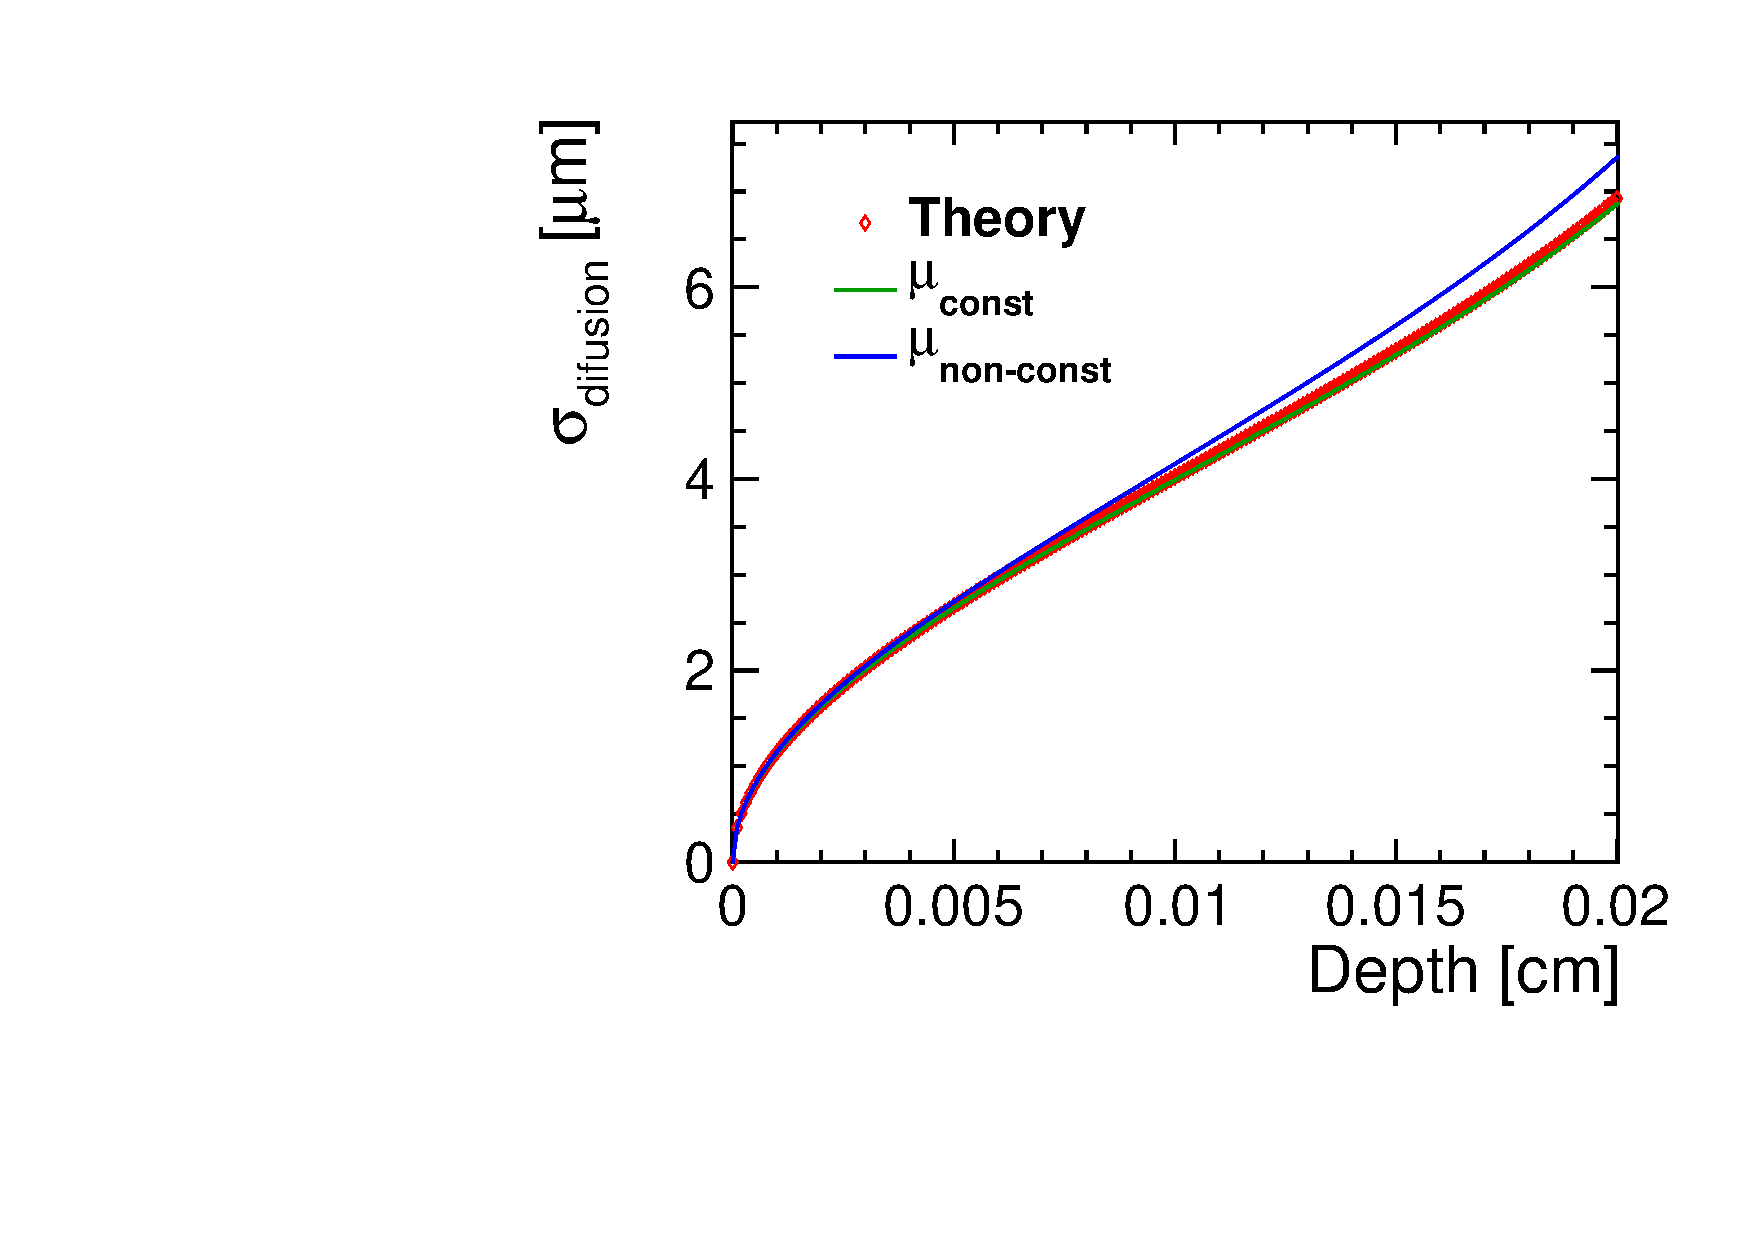
\includegraphics[width=\textwidth]{figures/ChargeSharing/B06_SigmaDiffusion.pdf}
    \caption{}\label{fig:}
  \end{subfigure} 
  \caption{The diffusion constant and spread for a constant mobility
    and a mobility which depends on the electric field. }\label{fig:}
\end{figure}

Comparing TCAD simulations and the charge sharing obtained by the
theoretical calculations gives us the following for a 200~\micron with
a depletion voltage of 30.31~V. Comparing for two different bias
voltages of 35~V and 50~V. In the case of the TCAD
simulations these results depend largely on the mesh divisions and
their locations. Both TCAD and theory assume a charge deposition of
80e- per \micron.

\begin{figure}[htbp]
  \centering
  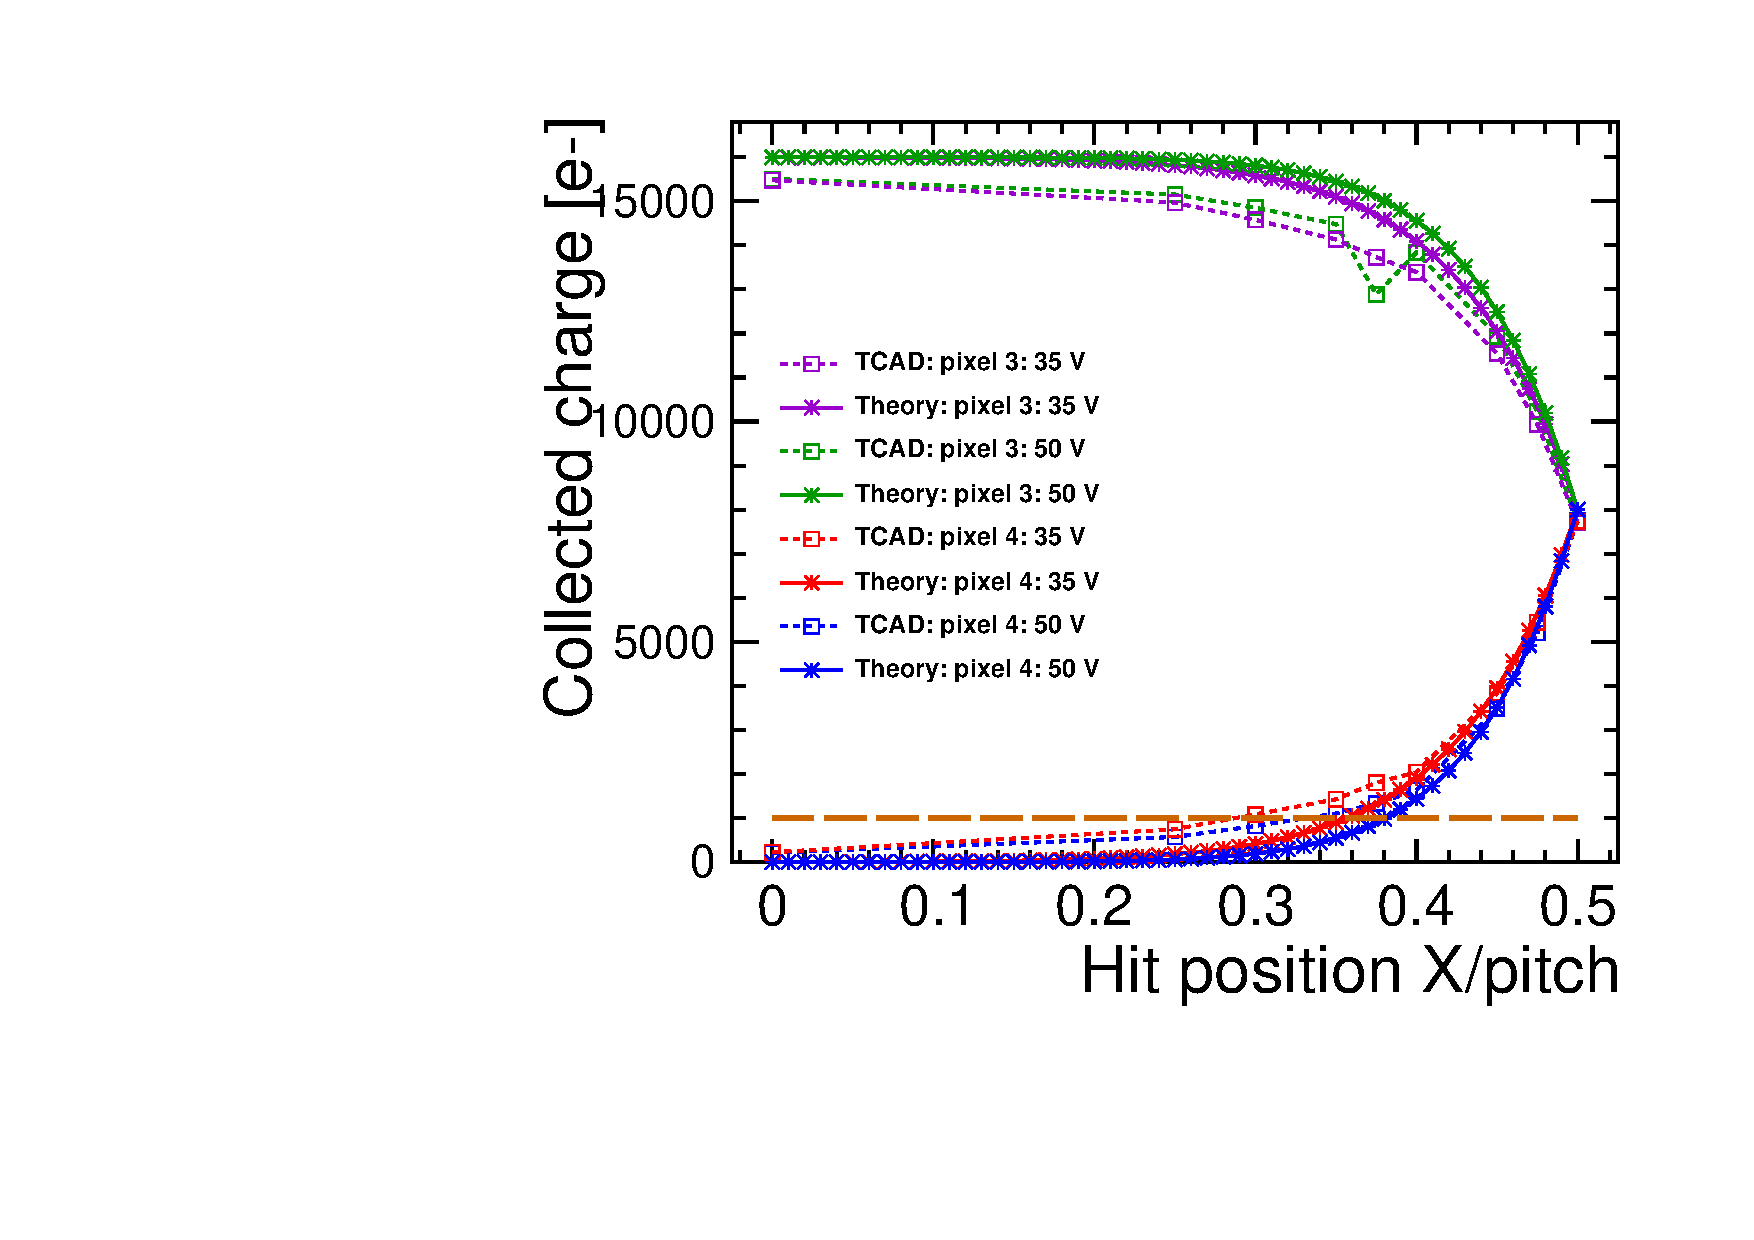
\includegraphics[width=0.5\textwidth]{figures/ChargeSharing/tcad_vs_theory.pdf}
  \caption{Diffusion comparing TCAD and theory.}\label{fig:}
\end{figure}


\section{Spatial resolution}

The spatial resolution of a pixel detector is mainly determined by the pixel
pitch. But this can be improved by the readout choice (binary or
analog), the threshold value, the charge sharing, thickness of the
detector and the reconstruction algorithm. The effect of the readout
is studied in the sections here-below.

\begin{figure}[htbp]
  \centering
  \begin{subfigure}[b]{0.3\textwidth}
    \centering
    \begin{tikzpicture}
      \draw[->, thick] (-2,0)--(2,0) node[right]{$x$};
      \draw[->, thick] (0, -0.5)--(0, 2) node[above]{$D\left(x\right)$};
      
      \draw[-] (-1.5, 1) -- (-1.5, 0) node[below]{${-p \over 2}$};
      \draw[-] (-1.5, 1) -- (1.5, 1);
      \draw[-] (1.5, 1) -- (1.5, 0) node[below]{${p \over 2}$};
      \node[] at (0.2, 1.2) {1};
    \end{tikzpicture}
    \caption{}\label{fig:SpatResBinary}
  \end{subfigure}\hfill
  \begin{subfigure}[b]{0.3\textwidth}
    \centering
    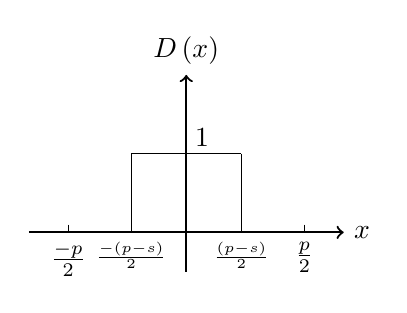
\begin{tikzpicture}
      \draw[->, thick] (-2,0)--(2,0) node[right]{$x$};
      \draw[->, thick] (0, -0.5)--(0, 2) node[above]{$D\left(x\right)$};
      
      \draw[-] (-0.7, 1) -- (-0.7, 0) node[below]{\tiny ${{-(p-s)}\over 2}$};
      \draw[-] (-0.7, 1) -- (0.7, 1);
      \draw[-] (0.7, 1) -- (0.7, 0) node[below]{\tiny ${(p-s)\over 2}$};
      \node[] at (0.2, 1.2) {1};
      \draw[-] (-1.5, 0.1) -- (-1.5, 0) node[below] {${-p \over 2}$};
      \draw[-] (1.5, 0.1) -- (1.5, 0) node[below] {${p \over 2}$};
    \end{tikzpicture}
    \caption{}\label{fig:SpatResBinaryChargeSharing}
  \end{subfigure}\hfill
  \begin{subfigure}[b]{0.3\textwidth}
    \centering
    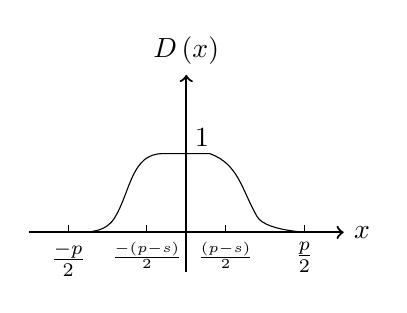
\begin{tikzpicture}
      \draw[->, thick] (-2,0)--(2,0) node[right]{$x$};
      \draw[->, thick] (0, -0.5)--(0, 2) node[above]{$D\left(x\right)$};
      
      \draw (-1.5,0) to[out=0, in=-120] (-0.9,0.2) to[out=60, in=180](-0.3, 1)--(0,1);
      \draw (0,1)--(0.3, 1) to [out=-20, in=120] (0.9,0.2) to[out=-60,
      in=0] (1.5,0);

      \draw[-] (-1.5, 0.1) -- (-1.5, 0) node[below] {${-p \over 2}$};
      \draw[-] (1.5, 0.1) -- (1.5, 0) node[below] {${p \over 2}$};

      \draw[-] (-0.5, 0.1) -- (-0.5, 0) node[below] {\tiny ${-(p-s) \over 2}$};
      \draw[-] (0.5, 0.1) -- (0.5, 0) node[below] {\tiny ${(p-s) \over 2}$};

      \node[] at (0.2, 1.2) {1};
    \end{tikzpicture}
    \caption{}\label{fig:SpatResAnaglogChargeSharing}
  \end{subfigure}
  \caption{(a) Binary readout. (b) Binary readout with charge
    sharing. (c) Analog readout with charge sharing.}\label{fig:SpatialResolution}
\end{figure}

The spatial resolution is defined by:
\begin{equation}
\sigma_{position}^2={{\int_{-p/2}^{p/2} \left(x_r-x_m\right)^2
    D\left(x_r\right) dx_r } \over { \int_{-p/2}^{p/2}
    D\left(x_r\right) dx_r }}\; ,
\label{eq:spatialRes}
\end{equation}

where $\sigma_{position}$ is the average distance between the real
impact position ($x_r$) and the measured position ($x_m$) of the
particle in a pixel.

\subsection{Binary readout}
For a binary readout, for a pixel centered at 0 and having a pitch
$p$, where only one pixel is fired per particle track the probability
density function $D\left(x\right)$ is illustrated in
Figure~\ref{fig:SpatResBinary}.  The average difference between the
real position ($x_r$) and the measured position ($x_m=0$) of the
particle in a pixel is calculated using Equation~\ref{eq:spatialRes}
\cite{Rossi:976471}:
\begin{equation}
\sigma_{position}^2={{\int_{-p/2}^{p/2} \left(x_r\right)^2
    1 dx_r } \over { \int_{-p/2}^{p/2}
    1 dx_r }}={p^2 \over 12} \; ,
\label{eq:spatialResBinary}
\end{equation}
which results in a spatial resolution of:
\begin{equation}
\sigma_{position}={p \over \sqrt{12}} \;.
\label{eq:sigmapos}
\end{equation}


\subsection{Binary readout and charge sharing}
The threshold of the readout electronics is usually set as low as
possible which can result in more than one pixel hit per particle
track. In this case, the charge is shared between two or more pixels
and this group is called a cluster. Multi-hit clusters improves the
resolution of
Equation~\ref{eq:spatialResBinary}. Figure~\ref{fig:SpatResBinaryChargeSharing}
illustrates the charge sharing between two pixels. If a track passes
close to the edge of a pixel (within a distance of $s\over 2$ close to
the edge), then the neighbouring pixel is also fired. For events
triggering single-hit events, the spatial resolution is given by:

\begin{equation}
\sigma_{position}^2={{\int_{-(p/2-s/2)}^{(p/2-s/2)} \left(x_r\right)^2
    1 dx_r } \over { \int_{-(p/2-s/2)}^{(p/2-s/2)}
    1 dx_r }}={(p-s)^2 \over 12} \; ,
\label{eq:spatialResCharge sharing_1hit}
\end{equation}

and for two-hit clusters, the spatial resolution is given by
\begin{equation}
\sigma_{position}={s \over \sqrt{12}} \; .
\label{eq:spatialResCharge sharing_2hit}
\end{equation}

The optimal average spatial resolution is obtained for $s=p/2$. This
means that the number of single-hit and multi-hit clusters is the
same. But, in this situation one is not able to distinguish between
one track triggering two pixels and two tracks hitting the sensor
within $2p$.

\subsection{Analog readout and charge sharing}
The spatial resolution can be improved more when an analog readout is
used that delivers a signal proportional to the collected charge as
illustrated in Figure~\ref{fig:SpatResAnaglogChargeSharing}. In this
case, for multi-hit clusters $\eta$-function as described
in~\cite{Belau:1983eh} is used to reconstruct the hit position within
the pixels. 
In the region where only one pixel fires, the resolution is still
limited to $(p-s)\over \sqrt{12}$.

The charge carriers follow the field lines to end-up on a certain
electrode. They are also subject to thermal diffusion which spreads
the charge cloud as it drifts through the silicon. The width of the
diffusion $\sigma_{diffusion}(z)$ (for simplicity called $\sigma(z)$) at depth $z$ is given by
Equation~\ref{eq:driftTimeIntegrated}.
The charge distribution at position $x_{hit}$ for a pixel extending from
$x_1$ to $x_2$ is:
\begin{equation}
Q(x_{hit}, z)= Q(z) {1\over{\sqrt{2 \pi \sigma^2(z)}}}
{\int_{x_1}^{x_2} e^{-({{x-x_{hit}}\over{\sqrt{2} \sigma(z)}})^2} } dx\; .
\label{eq:ChargeDistribution}
\end{equation}

By integrating Equation~\ref{eq:ChargeDistribution} over the whole
thickness of the detector, the charge deposited in a pixel at
coordinate $x_{hit}$ having coordinates $x_1$ and $x_2$ is given by:  
\begin{equation}
Q(x_{hit})= \int_{x_1}^{x_2}  \int_{0}^{d} {Q(z) \over {\sqrt{2 \pi
      \sigma^2(z)}} } e^{-({{x-x_{hit}}\over{\sqrt{2} \sigma(z)}})^2}
  dz \; dx\; .
\label{eq:ChargeDistribution_integrated_z}
\end{equation}


\section{Ramo's theorem: induced charge}
When a charge moves in the sensitive volume of a detector, a current
$i_s(t)$ flows instantaneously. \\ 
First, consider the simple example of a charge $q$ near an infinitely
large electrode with all the electric field lines terminating on the
electrode. The Gauss's law, for a surface $S$ surrounding the charge
is expressed as

\begin{equation}
\oint_{s} \vec{E} \cdot d\vec{a}=q\; .
\label{eq:GaussLaw}
\end{equation}

The induced charge obtained by integrating over a Gaussian surface
enclosing only the electrode is $-q$. \\
Considering two parallel electrodes with a charge $q$ in between as
showin in Figure~\ref{fig:InducedCharge_parallelPlates}. If the charge
is placed midway between the two parallel plates, it induces equal
charge of $-q/2$ on the both electrodes as half of the electric field
lines end up on the higher and the other half on the lower
electrode. When the charge moves towards the closer to a plate rather
than the other, the induced charge will be higher for the closer
plate. \\
The induced charge can not be observed directly but its change can be
measured when the two electrodes are connected in a closed circuit
(like a pixel detector) as it produces an induced current.

\begin{figure}[htbp]
  \centering
  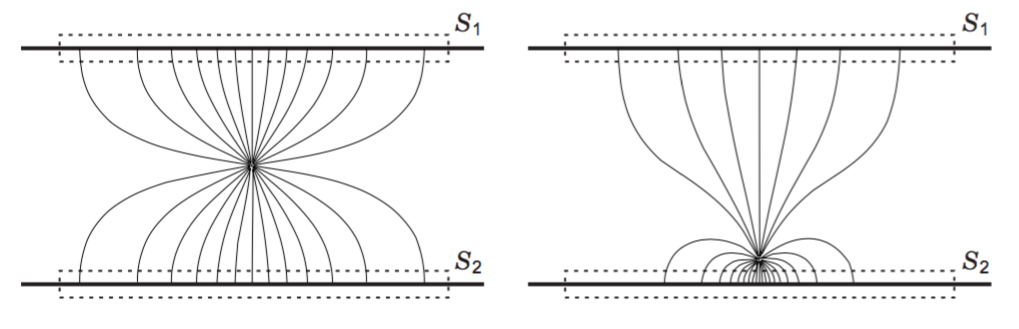
\includegraphics[width=0.8\textwidth]{figures/Ramo/InducedCharge_parallelPlates.png}
  \caption{The charge induced on two parallel plates depending on the
    position of the charge $q$. From~\cite{Spieler2005}.}
  \label{fig:InducedCharge_parallelPlates}
\end{figure}

Ramo's theorem describes the time evolution of the induced current
created in a detector. The induced current on the electrodes is
described as a function of the weighting potential $\Phi$ which
describes the coupling of a charge to an electrode. \\
The weighting potential is defined for a specific electrode. It is
obtained by setting the potential of the electrode to 1 and setting
all other electrodes to potential 0. Equation~\ref{eq:RamoCharge}
describes the induced charge $Q_k$ on electrode $k$ if a charge q moves along
any path from position $z_0$ to $z_p$.
\begin{equation}
    Q_{k}=q \cdot [\Phi_k(z_p)-\Phi_k(z_0)] \; .
   \label{eq:RamoCharge} 
  \end{equation}

 It is important to note that the weighting potential (field) is
 different than the electric potential (field). The electric field
 determines the drift trajectory and velocity of the charge carriers
 whereas the weighting field depends only on the geometry of the
 electrodes and defines how the charge motion induces a charge to a
 specific electrode. In the specific case of two-electrode configuration the
 electric and the weighting fields are the same. \\
In a TCAD simulation, the weighting field and potential are obtained
as shown in Figure~\ref{fig:RamoTCAD}. For this study the silicon
sensor has a thickness of 200~\micron and is over-depleted with a bias
voltage of \SI{50}{\volt} on the back-side. First, \SI{0}{\volt} is
applied to all the electrodes and then \SI{1}{\volt} is applied to the
electrode~$k$. By taking the difference between the two
configurations, the weighting potential and field are obtained.


\begin{figure}[htbp]
  \centering
  \begin{subfigure}[b]{0.49\textwidth}
    \centering
    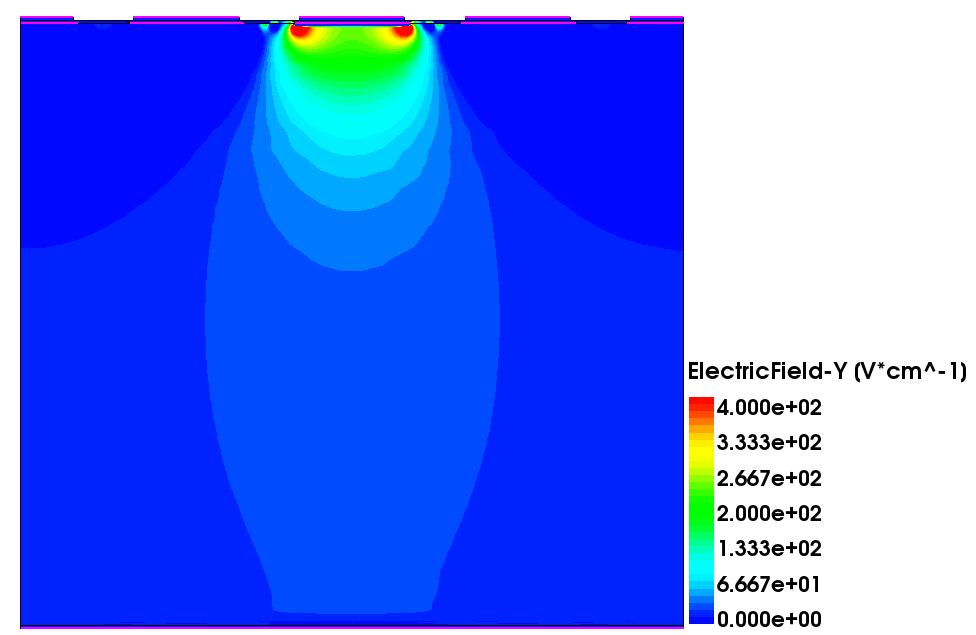
\includegraphics[width=\textwidth]{figures/Ramo/EfieldY_Ramo.png}
    \caption{Weighting field}\label{fig:WeightingFieldRamo}
  \end{subfigure}\hfill
  \begin{subfigure}[b]{0.49\textwidth}
    \centering
    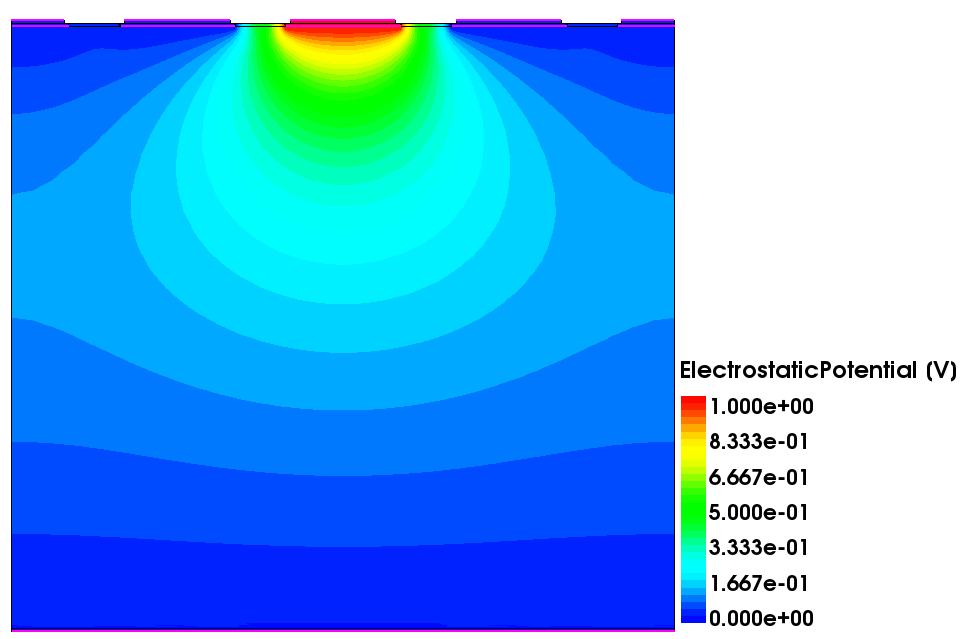
\includegraphics[width=\textwidth]{figures/Ramo/RamoPotential.png}
    \caption{Weighting potential}\label{fig:WeightingPotentialRamo}
  \end{subfigure} 
  \caption{The weighting field and potential.}\label{fig:RamoTCAD}
\end{figure}

The weighting potential for different positions on the
x-axis is shown in Figure~\ref{fig:RamoTCADCuts}. Since, the total
charge collected by the electrode $k$ depends only on the positions
$z_0$ and $z_p$, in the absence of the radiation-induced damages
(which would affect the distributions of the electric and weighting
fields), the Ramo theorem can be neglected.

\begin{figure}[htbp]
  \centering
  \begin{subfigure}[b]{0.49\textwidth}
    \centering
    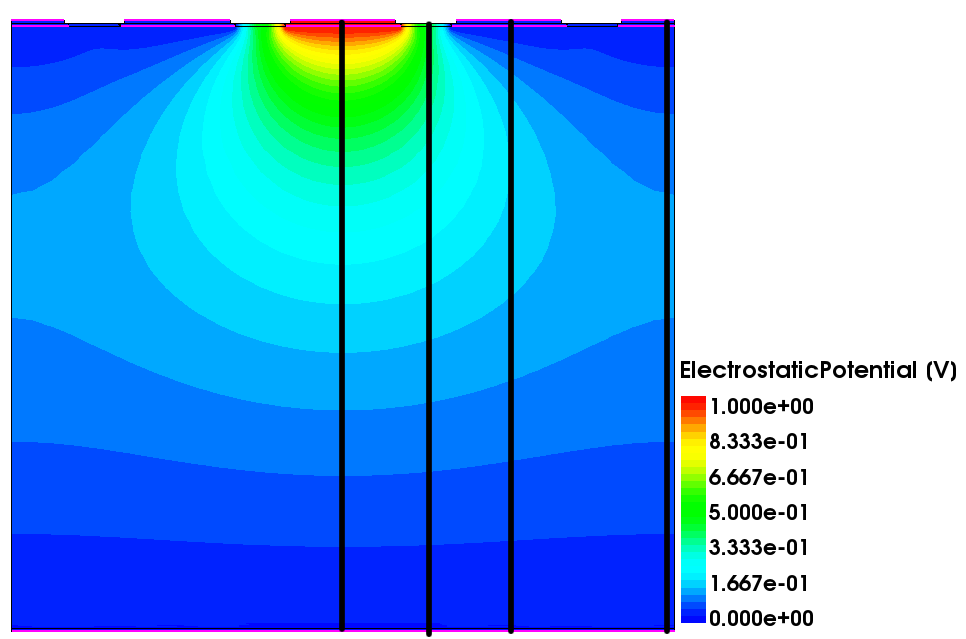
\includegraphics[width=\textwidth]{figures/Ramo/RamoPotential_cuts.png}
    \caption{}\label{fig:RamoPotentialCuts}
  \end{subfigure}\hfill
  \begin{subfigure}[b]{0.49\textwidth}
    \centering
    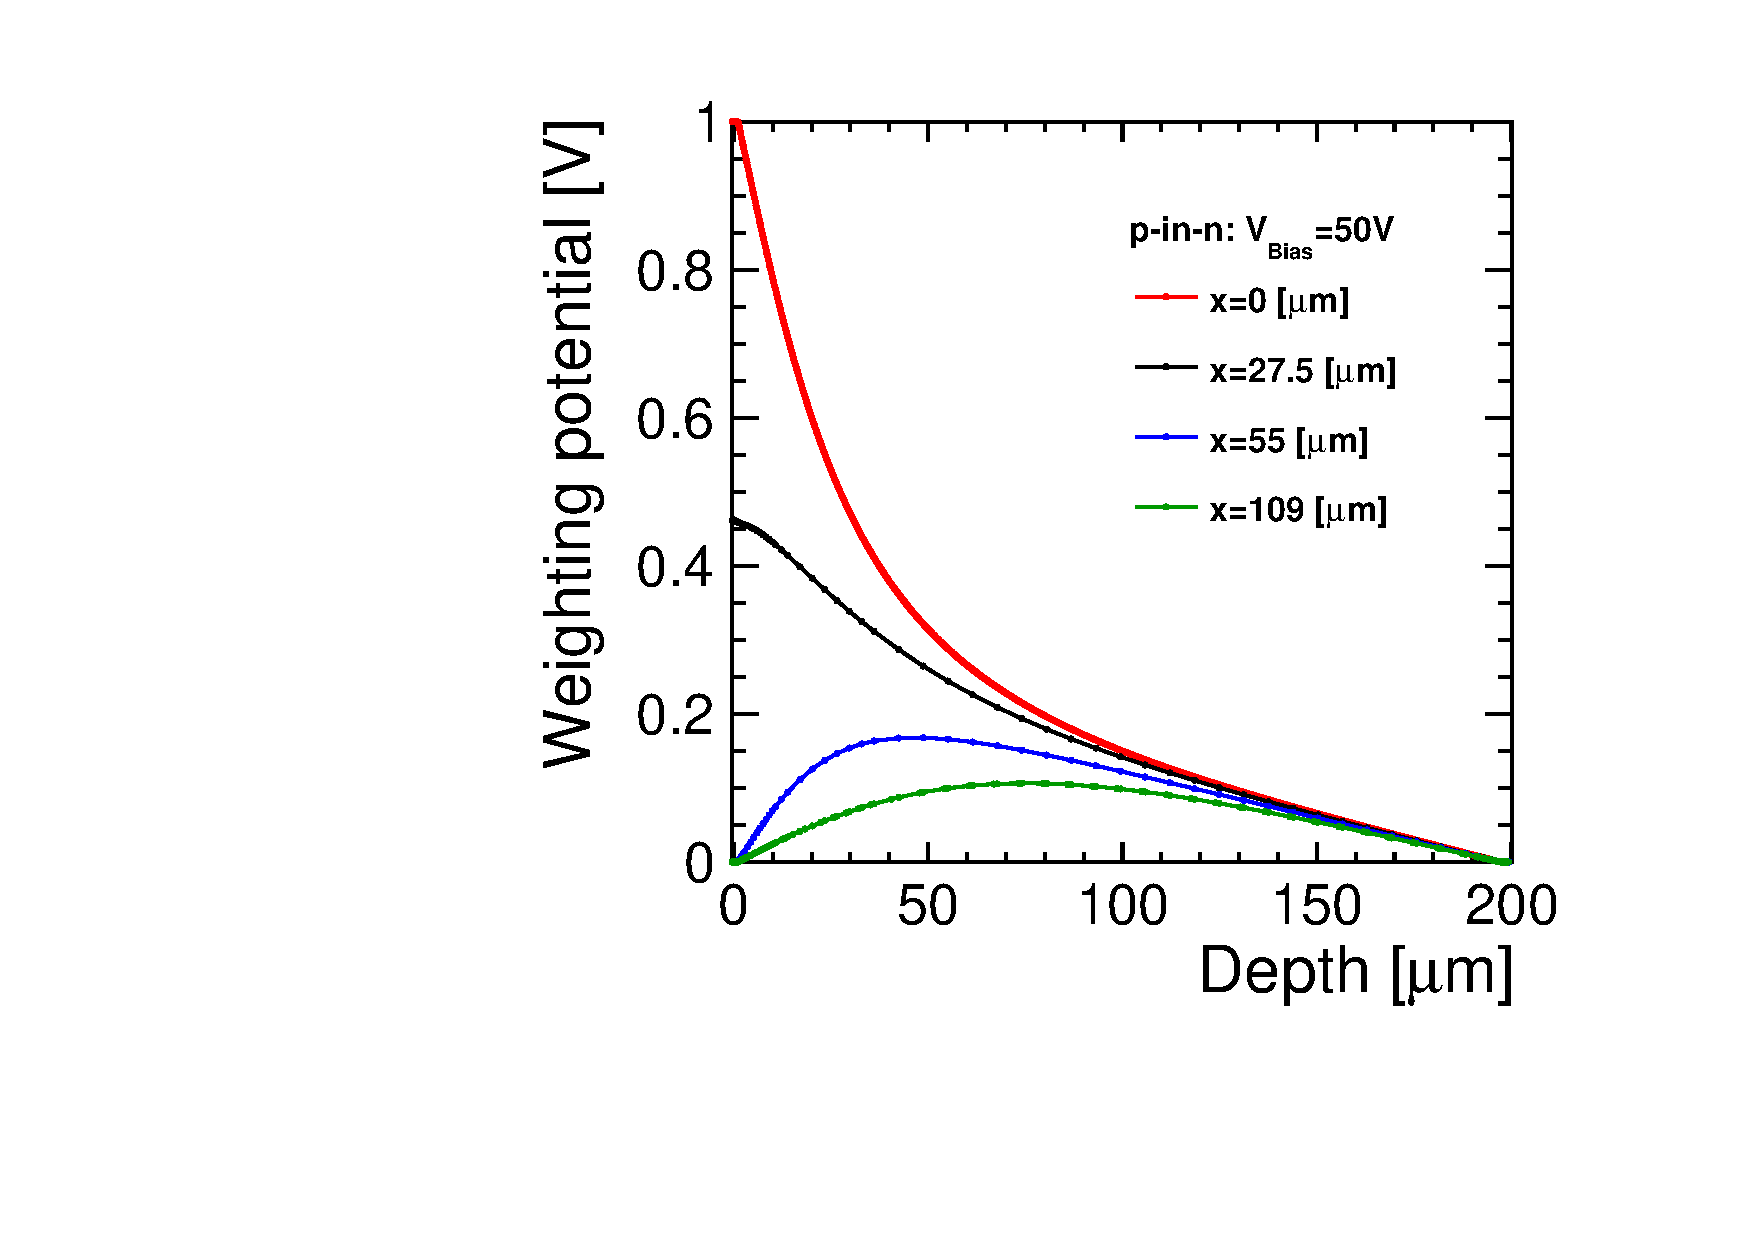
\includegraphics[width=\textwidth]{figures/Ramo/WeightingPotential_1D.pdf}
    \caption{}\label{fig:RamoPotentialCuts1D}
  \end{subfigure} 
  \caption{The weighting potential for different positions on the x-axis.}\label{fig:RamoTCADCuts}
\end{figure}



%% --------- Recycle text --------- %%
% \section{Detector systems}

% Figure~\ref{fig:basicDetectorFunction}, schematically summarises the sequence of basic detector functions.


% \begin{figure}[htbp]
%   \centering
%   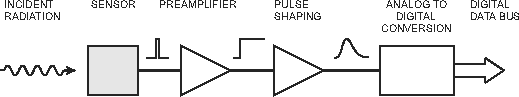
\includegraphics[width=\textwidth]{figures/basicDetectorFunction.png}
%   \caption{The sequence of basic detector functions. From~\cite{Spieler2005}.}
%   \label{fig:basicDetectorFunction}
% \end{figure}


% \subsection{Sensor} 
% A silicon sensor, converts the energy deposited by a particle to an electric signal by producing electron-hole pairs. By applying an electric field to the sensor, the produced pairs are con
% \subsection{Preamplifier}
% \subsection{Pulse shaper}
% \subsection{Digitiser}

%% --------------------------------------------------- %%
% Carriers move in random direction due to the thermal energy. \\
% Material-dependent diffusion constant given by the Einstein equation:  

% \begin{equation}
%   D_{b}={{k_{B} \cdot T \cdot \mu_{c}} \over {e}}
% \end{equation}
% where \(k=8.617 3324\) is the Boltzman constant.

% \begin{equation}
%   \sigma_{diffusion}=\sqrt{2 \cdot D_{b} \cdot t_{c}}
% \end{equation}



